\documentclass[11pt,a4paper]{ctexart}
% Shared preamble for the assignment reports. Use with:
%   \documentclass[11pt,a4paper]{ctexart}  (XeLaTeX)
%   % Shared preamble for the assignment reports. Use with:
%   \documentclass[11pt,a4paper]{ctexart}  (XeLaTeX)
%   % Shared preamble for the assignment reports. Use with:
%   \documentclass[11pt,a4paper]{ctexart}  (XeLaTeX)
%   \input{../common/preamble.tex}
\usepackage[margin=2.3cm]{geometry}
\setmainfont{texgyretermes}[Extension=.otf,UprightFont=*-regular,BoldFont=*-bold,ItalicFont=*-italic,BoldItalicFont=*-bolditalic]
\setsansfont{texgyreheros}[Extension=.otf,UprightFont=*-regular,BoldFont=*-bold,ItalicFont=*-italic,BoldItalicFont=*-bolditalic]
\setmonofont{texgyrecursor}[Extension=.otf,UprightFont=*-regular,BoldFont=*-bold,ItalicFont=*-italic,BoldItalicFont=*-bolditalic]
\usepackage{amsmath,amssymb,mathtools,bm}
\usepackage{graphicx}
\usepackage{booktabs,multirow,makecell,array,tabularx}
\usepackage[table]{xcolor}
\usepackage[most]{tcolorbox}
\usepackage{enumitem}
\usepackage{listings}
\usepackage{subcaption}
\usepackage{siunitx}
\usepackage[hidelinks]{hyperref}
\usepackage[nameinlink,noabbrev]{cleveref}
\usepackage{float}

\setlength{\emergencystretch}{3em}
\linespread{1.15}
\setlist{leftmargin=*,itemsep=2pt,topsep=3pt}
\graphicspath{{figures/}}

\crefname{figure}{图}{图}
\crefname{table}{表}{表}
\crefname{section}{第}{第}
\creflabelformat{section}{#2#1#3 节}
\crefname{equation}{式}{式}
\crefformat{equation}{式~(#2#1#3)}

\lstset{basicstyle=\ttfamily\footnotesize,columns=fullflexible,breaklines=true,frame=single,
  framerule=0.3pt,rulecolor=\color{black!40},backgroundcolor=\color{black!3},
  keywordstyle=\color{blue!60!black}\bfseries,commentstyle=\color{green!40!black},
  numbers=left,numberstyle=\tiny\color{black!50},xleftmargin=1.5em}

% Interview boxes: question, model answer, common wrong answer.
\newtcolorbox{iqbox}[1]{enhanced,breakable,colback=blue!3,colframe=blue!45!black,boxrule=0.5pt,arc=1.5pt,
  left=4pt,right=4pt,top=3pt,bottom=3pt,fonttitle=\bfseries\small,title={面试追问：#1}}
\newtcolorbox{findingbox}[1][]{enhanced,breakable,colback=green!3,colframe=green!40!black,boxrule=0.5pt,arc=1.5pt,
  left=4pt,right=4pt,top=3pt,bottom=3pt,fonttitle=\bfseries\small,title={结论#1}}
\newtcolorbox{caveatbox}{enhanced,breakable,colback=orange!4,colframe=orange!60!black,boxrule=0.5pt,arc=1.5pt,
  left=4pt,right=4pt,top=3pt,bottom=3pt,fonttitle=\bfseries\small,title={不能推出的结论}}

\newcommand{\authorline}{ShaneLiu04\thanks{GitHub: \url{https://github.com/ShaneLiu04}。代码与原始指标：\url{https://gitee.com/liu-xingyan04/mlsys-infra}。本文基于公开课程材料独立完成，与课程团队无隶属关系。}}

\usepackage[margin=2.3cm]{geometry}
\setmainfont{texgyretermes}[Extension=.otf,UprightFont=*-regular,BoldFont=*-bold,ItalicFont=*-italic,BoldItalicFont=*-bolditalic]
\setsansfont{texgyreheros}[Extension=.otf,UprightFont=*-regular,BoldFont=*-bold,ItalicFont=*-italic,BoldItalicFont=*-bolditalic]
\setmonofont{texgyrecursor}[Extension=.otf,UprightFont=*-regular,BoldFont=*-bold,ItalicFont=*-italic,BoldItalicFont=*-bolditalic]
\usepackage{amsmath,amssymb,mathtools,bm}
\usepackage{graphicx}
\usepackage{booktabs,multirow,makecell,array,tabularx}
\usepackage[table]{xcolor}
\usepackage[most]{tcolorbox}
\usepackage{enumitem}
\usepackage{listings}
\usepackage{subcaption}
\usepackage{siunitx}
\usepackage[hidelinks]{hyperref}
\usepackage[nameinlink,noabbrev]{cleveref}
\usepackage{float}

\setlength{\emergencystretch}{3em}
\linespread{1.15}
\setlist{leftmargin=*,itemsep=2pt,topsep=3pt}
\graphicspath{{figures/}}

\crefname{figure}{图}{图}
\crefname{table}{表}{表}
\crefname{section}{第}{第}
\creflabelformat{section}{#2#1#3 节}
\crefname{equation}{式}{式}
\crefformat{equation}{式~(#2#1#3)}

\lstset{basicstyle=\ttfamily\footnotesize,columns=fullflexible,breaklines=true,frame=single,
  framerule=0.3pt,rulecolor=\color{black!40},backgroundcolor=\color{black!3},
  keywordstyle=\color{blue!60!black}\bfseries,commentstyle=\color{green!40!black},
  numbers=left,numberstyle=\tiny\color{black!50},xleftmargin=1.5em}

% Interview boxes: question, model answer, common wrong answer.
\newtcolorbox{iqbox}[1]{enhanced,breakable,colback=blue!3,colframe=blue!45!black,boxrule=0.5pt,arc=1.5pt,
  left=4pt,right=4pt,top=3pt,bottom=3pt,fonttitle=\bfseries\small,title={面试追问：#1}}
\newtcolorbox{findingbox}[1][]{enhanced,breakable,colback=green!3,colframe=green!40!black,boxrule=0.5pt,arc=1.5pt,
  left=4pt,right=4pt,top=3pt,bottom=3pt,fonttitle=\bfseries\small,title={结论#1}}
\newtcolorbox{caveatbox}{enhanced,breakable,colback=orange!4,colframe=orange!60!black,boxrule=0.5pt,arc=1.5pt,
  left=4pt,right=4pt,top=3pt,bottom=3pt,fonttitle=\bfseries\small,title={不能推出的结论}}

\newcommand{\authorline}{ShaneLiu04\thanks{GitHub: \url{https://github.com/ShaneLiu04}。代码与原始指标：\url{https://gitee.com/liu-xingyan04/mlsys-infra}。本文基于公开课程材料独立完成，与课程团队无隶属关系。}}

\usepackage[margin=2.3cm]{geometry}
\setmainfont{texgyretermes}[Extension=.otf,UprightFont=*-regular,BoldFont=*-bold,ItalicFont=*-italic,BoldItalicFont=*-bolditalic]
\setsansfont{texgyreheros}[Extension=.otf,UprightFont=*-regular,BoldFont=*-bold,ItalicFont=*-italic,BoldItalicFont=*-bolditalic]
\setmonofont{texgyrecursor}[Extension=.otf,UprightFont=*-regular,BoldFont=*-bold,ItalicFont=*-italic,BoldItalicFont=*-bolditalic]
\usepackage{amsmath,amssymb,mathtools,bm}
\usepackage{graphicx}
\usepackage{booktabs,multirow,makecell,array,tabularx}
\usepackage[table]{xcolor}
\usepackage[most]{tcolorbox}
\usepackage{enumitem}
\usepackage{listings}
\usepackage{subcaption}
\usepackage{siunitx}
\usepackage[hidelinks]{hyperref}
\usepackage[nameinlink,noabbrev]{cleveref}
\usepackage{float}

\setlength{\emergencystretch}{3em}
\linespread{1.15}
\setlist{leftmargin=*,itemsep=2pt,topsep=3pt}
\graphicspath{{figures/}}

\crefname{figure}{图}{图}
\crefname{table}{表}{表}
\crefname{section}{第}{第}
\creflabelformat{section}{#2#1#3 节}
\crefname{equation}{式}{式}
\crefformat{equation}{式~(#2#1#3)}

\lstset{basicstyle=\ttfamily\footnotesize,columns=fullflexible,breaklines=true,frame=single,
  framerule=0.3pt,rulecolor=\color{black!40},backgroundcolor=\color{black!3},
  keywordstyle=\color{blue!60!black}\bfseries,commentstyle=\color{green!40!black},
  numbers=left,numberstyle=\tiny\color{black!50},xleftmargin=1.5em}

% Interview boxes: question, model answer, common wrong answer.
\newtcolorbox{iqbox}[1]{enhanced,breakable,colback=blue!3,colframe=blue!45!black,boxrule=0.5pt,arc=1.5pt,
  left=4pt,right=4pt,top=3pt,bottom=3pt,fonttitle=\bfseries\small,title={面试追问：#1}}
\newtcolorbox{findingbox}[1][]{enhanced,breakable,colback=green!3,colframe=green!40!black,boxrule=0.5pt,arc=1.5pt,
  left=4pt,right=4pt,top=3pt,bottom=3pt,fonttitle=\bfseries\small,title={结论#1}}
\newtcolorbox{caveatbox}{enhanced,breakable,colback=orange!4,colframe=orange!60!black,boxrule=0.5pt,arc=1.5pt,
  left=4pt,right=4pt,top=3pt,bottom=3pt,fonttitle=\bfseries\small,title={不能推出的结论}}

\newcommand{\authorline}{ShaneLiu04\thanks{GitHub: \url{https://github.com/ShaneLiu04}。代码与原始指标：\url{https://gitee.com/liu-xingyan04/mlsys-infra}。本文基于公开课程材料独立完成，与课程团队无隶属关系。}}

\graphicspath{{../../solutions/cs229s/project2-kv-speculative/artifacts/figures/}}

\title{CS229S Project 2 实验报告：\\GPT-2 上的 KV Cache、CUDA Graph 与推测解码（CPU 原型 + RTX 5090 实测）}
\author{\authorline}
\date{2026 年 10 月}

\begin{document}
\maketitle

\begin{abstract}
本报告完成 Stanford CS229S（Fall 2023）Project 2 的两大部分：给 nanoGPT 风格的解码器加 KV cache，并实现
Leviathan/Chen 的推测解码（speculative decoding），测量加速并与理论对照。实验分两层：
（1）CPU 原型：在合成语法上训练的 4 层 target 与 1 层 draft，用来做严格的单元测试（float64 下 KV 与无 cache 的 logits 差 $\le 10^{-9}$，
接受-拒绝采样 60{,}000 次的卡方检验）；（2）GPU 实测：自己写的 GPT-2 前向直接加载 HuggingFace 的
gpt2 / gpt2-medium / gpt2-large / gpt2-xl 真实权重，在 RTX 5090 上实现无 cache、预分配静态 KV cache、CUDA Graph decode 三个版本，
以及带 KV 回滚的 GPU 推测解码（贪心与采样）。
主要结论：（a）fp32 下 gpt2-large / gpt2-xl 的 logits 与 HF 的最大差为 $4.2\times10^{-5}$ / $4.6\times10^{-5}$，4 个模型三种实现的贪心输出 60/60 逐 token 相同；
（b）gpt2-xl 在上下文 1024 时每 token 延迟从无 cache 的 20.62 ms 降到 KV + CUDA Graph 的 4.22 ms，但 batch 1 decode 仍是 roofline 下界的约 1.9 倍，差值与层数成正比（每层约 30--41 µs 的 kernel 固定开销）；
短上下文时 eager KV cache 甚至比无 cache 更慢；（c）KV cache 的 \texttt{memory\_allocated} 在 58/63 个配置上与公式逐字节相等；
（d）gpt2→gpt2-xl 推测解码贪心实测 1.631 倍、$T{=}1$ 为 1.454 倍，接受率 $\hat\alpha$ 与 $1-\mathrm{TV}$ 吻合，每次调用 token 数与 $(1-\alpha^{\gamma+1})/(1-\alpha)$ 的差 $<1\%$（采样），
用实测 $c{=}0.138$、$v{\approx}1.11$ 代入的预测与实测之比为 0.87--1.00；（e）fp32 下推测解码贪心输出与 target 120/120 一致，采样版 4000 次对精确 target 分布的卡方 $p$ 值 0.657，对 draft 分布 $8.9\times10^{-168}$；
（f）数据展示了加速转为减速的三种方式：$\gamma$ 过大（gpt2-large $T{=}1,\gamma\ge5$）、更大的 draft（gpt2-medium 的 $c{=}0.308$）、更大的 batch（验证不再免费）。
\end{abstract}

\tableofcontents
\newpage

\section{背景与作业要求}

CS229S Project 2 的官方要求可以概括为三件事：
\begin{enumerate}
  \item \textbf{KV cache}：在 nanoGPT 上实现 KV cache，比较有/无 cache 的生成速度，并分析显存开销；
  \item \textbf{推测解码~\cite{leviathan}}：用小模型（draft）提议 $\gamma$ 个 token，大模型（target）一次 forward 验证，
        实现接受-拒绝~\cite{chen}采样，测量接受率与加速比；
  \item \textbf{分析}：用 roofline~\cite{roofline} / 访存模型解释为什么 decode 是 memory-bound~\cite{pope}，为什么推测解码在 GPU 上有效、什么时候失效。
\end{enumerate}
\Cref{tab:map} 把官方各部分映射到本仓库的实现。

\begin{table}[H]
\centering\small
\caption{官方作业 → 本仓库实现}\label{tab:map}
\begin{tabularx}{\linewidth}{>{\raggedright\arraybackslash}p{2.3cm} >{\raggedright\arraybackslash}X >{\raggedright\arraybackslash}X}
\toprule
官方部分 & CPU 原型（\texttt{code/kvspec}） & GPU 实测（\texttt{gpu/}） \\
\midrule
nanoGPT + KV cache & \texttt{model.py}：预分配 $(L,B,H,T_{\max},d_h)$ 缓冲区，\texttt{length} 回滚 &
  \texttt{gpt2\_fast.py}：同样的静态 cache，加载 HF GPT-2~\cite{gpt2} 权重；eager 与 CUDA Graph 两种 decode \\
正确性 & float64 下 KV 与无 cache logits 差 $\le10^{-9}$ & fp32 logits 对 HF \texttt{transformers}；贪心输出逐 token 比较 \\
推测解码 & \texttt{speculative.py}：numpy 接受-拒绝 & \texttt{SpecEngine}：全在 GPU 上的接受-拒绝，每轮只同步一次 \\
分布无偏 & 显式 $p,q$，60{,}000 次卡方检验 & 真实 gpt2→gpt2-large，4000 次采样对精确 $p$ 做卡方检验 \\
理论对照 & $(1-\alpha^{\gamma+1})/(1-\alpha)$，$c$ 实测 & 同上 + \texttt{mlsys\_calc.decode\_step\_time} roofline 预测 \\
显存 & 公式 & \texttt{torch.cuda.memory\_allocated} 实测 vs 公式 \\
\bottomrule
\end{tabularx}
\end{table}

\section{实验环境}

\begin{itemize}
  \item \textbf{CPU 原型}：Windows Server，Intel 4 物理核 / 8 逻辑核（与其他任务共享），Python 3.12.10，torch 2.6.0+cpu；训练 8 线程、decode 计时 1 线程（\texttt{meta.json}）。
  \item \textbf{GPU}：AutoDL 上的 NVIDIA GeForce RTX 5090（sm\_120，170 SM，32 GB GDDR7，\texttt{hw.jsonl} 报告 33.67 GB 可见），
        torch 2.8.0+cu128，CUDA 12.8，transformers 5.21.0（仅用于对照 logits）。GPU 作业通过共享 \texttt{flock} 串行，避免与其他实验互相干扰；
        进程绑定 2 个 CPU 核（\texttt{taskset -c 41,43}）。
  \item \textbf{实测硬件峰值}（\texttt{hw.jsonl}）：2 GiB \texttt{copy\_} 的有效带宽 1522 GB/s（读+写各算一次）；
        fp16 GEMM $8192^3$ 达到 223.4 TFLOP/s。后文所有 roofline 预测都用这两个实测值构造
        \texttt{mlsys\_calc.GPU("RTX 5090 (measured)", ...)}，而不是规格书上的 1.79 TB/s。
  \item \textbf{数据}：推测解码与正确性检查的 prompt 取自 WikiText-2~\cite{wikitext}（raw，test split）的 GPT-2 token 流，随机截取 64-token 窗口；
        推测解码主实验 100 个 prompt，每个生成 64 个新 token。
  \item \textbf{精度}：正确性对照用 fp32（关闭 TF32），所有计时用 fp16。
\end{itemize}

\section{方法与实现}

\subsection{GPT-2 前向与权重加载}
HF 的 GPT-2 用 \texttt{Conv1D}，权重形状是 $(d_{in}, d_{out})$；我们直接读 \texttt{model.safetensors}，转置成 \texttt{F.linear} 的
$(d_{out}, d_{in})$ 布局并 \texttt{contiguous()}，LM head 与 \texttt{wte} 绑定，GELU 用 tanh 近似（即 HF 的 \texttt{gelu\_new}）。
\Cref{lst:fwd} 是一层的核心代码：三种 attention 路径共用一套线性层。

\begin{lstlisting}[language=Python,caption={\texttt{gpu/gpt2\_fast.py}：一层的 forward，三种 KV 路径},label=lst:fwd]
qkv = F.linear(_ln(x, l1w, l1b), qkvw, qkvb).view(B, t, 3, H, hd)
q, k, v = (z.transpose(1, 2) for z in qkv.unbind(2))
if cache is None:                       # (a) no cache: recompute the whole prefix
    y = F.scaled_dot_product_attention(q, k, v, is_causal=True)
elif pos is None:                       # (b) eager KV: write slice, attend to prefix
    cache.k[i, :, :, s:s + t] = k; cache.v[i, :, :, s:s + t] = v
    y = F.scaled_dot_product_attention(q, cache.k[i, :, :, :s+t], cache.v[i, :, :, :s+t], attn_mask=mask)
else:                                   # (c) static, CUDA-graph-safe: position is a device tensor
    cache.k[i].index_copy_(2, positions, k); cache.v[i].index_copy_(2, positions, v)
    y = sdpa_or_bmm(q, cache.k[i, :, :, :t_attn], cache.v[i, :, :, :t_attn], mask)
x = x + F.linear(y.transpose(1, 2).reshape(B, t, C), ow, ob)
x = x + F.linear(F.gelu(F.linear(_ln(x, l2w, l2b), fcw, fcb), approximate="tanh"), prw, prb)
\end{lstlisting}

\subsection{静态 KV cache 与 CUDA Graph}
KV cache 预分配为 $(L, B, H, T_{\max}, d_h)$ 的两个张量，\texttt{length} 指出有效前缀；推测解码拒绝 draft 时只需把 \texttt{length} 调小（回滚），不搬数据。
CUDA Graph 要求每次 replay 的张量地址与形状都不变，所以静态路径把「当前位置」做成一个 0 维 device 张量 \texttt{pos}，
写 cache 用 \texttt{index\_copy\_}，attention 在固定长度 $t_{\text{attn}}$ 的前缀上做，并用 \texttt{arange(t\_attn) <= positions} 的 mask 屏蔽未来位置。
graph 的 warm-up 和 capture 会在位置 $[0,t)$ 写入垃圾 K/V，所以必须\emph{先 capture、再 prefill}；prefill 会覆盖这些位置，而 mask 保证无效位置永远不被读到。

\begin{lstlisting}[language=Python,caption={\texttt{GraphStep}：一次 capture，之后每步只做两次小拷贝 + replay}]
self.idx = torch.zeros(B, t, dtype=torch.long, device=dev)
self.pos = torch.zeros((), dtype=torch.long, device=dev)
... warm-up on a side stream ...
with torch.cuda.graph(self.graph):
    self.out = model.forward(self.idx, cache, self.pos, self.t_attn)
def __call__(self, idx, pos):
    self.idx.copy_(idx); self.pos.fill_(pos); self.graph.replay(); return self.out
\end{lstlisting}

静态路径有两种 attention 实现：\texttt{sdpa}（PyTorch 的 \texttt{scaled\_dot\_product\_attention} 带 bool mask）和
\texttt{bmm}（显式 $QK^\top$、softmax、$PV$ 三个算子）。后者是在实验中发现前者在 batch 1 decode 时随上下文变慢之后加的（见 \cref{sec:lat}）。

\subsection{GPU 推测解码}
\texttt{SpecEngine} 为一对 (target, draft) 和固定的 $\gamma$ 预先 capture 四个 graph：target 的 $t{=}1$（基线）与 $t{=}\gamma{+}1$（验证），
draft 的 $t{=}1$ 与 $t{=}2$（draft 每轮最多缺 2 个 token：全部接受时缺 $x_\gamma$ 和 bonus token）。
每轮的流程：draft 自回归提议 $\gamma$ 个 token（采样在 GPU 上，不同步）；target 对 $[\text{seq}_{-1}, x_1..x_\gamma]$ 做一次 forward；
接受-拒绝全在 GPU 上算完后用一次 \texttt{tolist()} 同步取回 $(n_{acc}, \text{next}, \text{overlap})$。缓存不变量：每轮开始时 target cache 恰好存
\texttt{seq[:-1]}，draft cache 存 \texttt{seq} 的一个前缀（缺 1 或 2 个 token）。

\begin{lstlisting}[language=Python,caption={\texttt{accept\_reject\_torch}：无主机同步的接受-拒绝}]
ratio = p[r, drafts] / q[r, drafts]                     # p: (g+1,V) target, q: (g,V) draft
u = torch.rand(g, device=p.device, generator=gen)
n_acc = torch.cumprod((u < ratio).long(), 0).sum()      # index of first rejection
resid = torch.cat([(p[:g] - q).clamp_min(0), p[g:]])[n_acc]   # norm(max(p-q,0)) or bonus p_g
nxt = torch.multinomial(resid / resid.sum(), 1, generator=gen)[0]
\end{lstlisting}

贪心版本把接受条件换成 $x_i = \arg\max p_i$，第一个不一致处取 target 的 argmax。

\subsection{接受率 $\alpha$ 的定义}
沿用 CPU 版 README 的结论：一轮里第一次拒绝之后的 draft 从未被检验，所以 $\alpha$ 必须用
$\hat\alpha = \frac{\#\text{accepted}}{\#\text{accepted} + \#\text{rejections}}$（截断几何分布的极大似然估计），
而不是 $\#\text{accepted}/\#\text{proposed}$。采样模式下还记录 $\mathbb{E}[\sum_x \min(p,q)] = 1-\mathrm{TV}(p,q)$，这是 Leviathan 定义的 $\alpha$，应与 $\hat\alpha$ 一致。

\subsection{理论模型}
设每次 draft forward 的代价是 target 单 token forward 的 $c$ 倍，target 验证 $\gamma{+}1$ 个 token 的代价是单 token 的 $v$ 倍，则
\begin{equation}
\mathbb{E}[\text{tokens/round}] = \frac{1-\alpha^{\gamma+1}}{1-\alpha}, \qquad
S(\gamma) = \frac{\mathbb{E}[\text{tokens/round}]}{\gamma c + v}.
\label{eq:spec}
\end{equation}
$v{=}1$ 时就是 \texttt{mlsys\_calc.speculative\_speedup}。decode 一步的 roofline 下界来自 \texttt{mlsys\_calc.decode\_step\_time}：
\begin{equation}
t_{\text{step}} \ge \max\!\Big(\frac{2NB + 4LdTB}{P_{\text{peak}}},\ \frac{2N + 2\cdot 2LdTB}{BW}\Big),
\label{eq:roof}
\end{equation}
其中 $N$ 为参数量（含绑定的词嵌入），$B$ 为 batch，$T$ 为上下文长度，fp16 每元素 2 字节，KV 每 token 每层 $2d$ 个元素。

\section{实验结果}

\subsection{CPU 原型：KV cache 与推测解码（已有部分）}

CPU 原型的 target 有 796{,}928 个参数（4 层 $\times$ 128 宽），draft 29{,}712 个（1 层 $\times$ 48 宽），在 64 个随机「单词」组成的稀疏 bigram 合成语法上训练
（\texttt{models.json}）。\Cref{fig:cpu-kv} 左图是单步延迟：不用 cache 时第 $t$ 步要对 $t$ 个 token 做完整 forward，延迟从位置 16 的 2.27 ms 线性涨到位置 1008 的 59.0 ms；
KV cache 每步只算 1 个 token，从 1.42 ms 缓慢涨到 2.25 ms（attention 的 $O(t)$ 部分）。右图是总耗时：T 从 512 到 1024 时无 cache 涨 4.27 倍（$\sim T^2$），
KV 涨 2.15 倍（$\sim T$）；T=1024 时 KV 的生成速度 499.2 tok/s，是无 cache（38.9 tok/s）的 12.82 倍（\texttt{kv\_timing.csv}）。

\begin{figure}[H]
\centering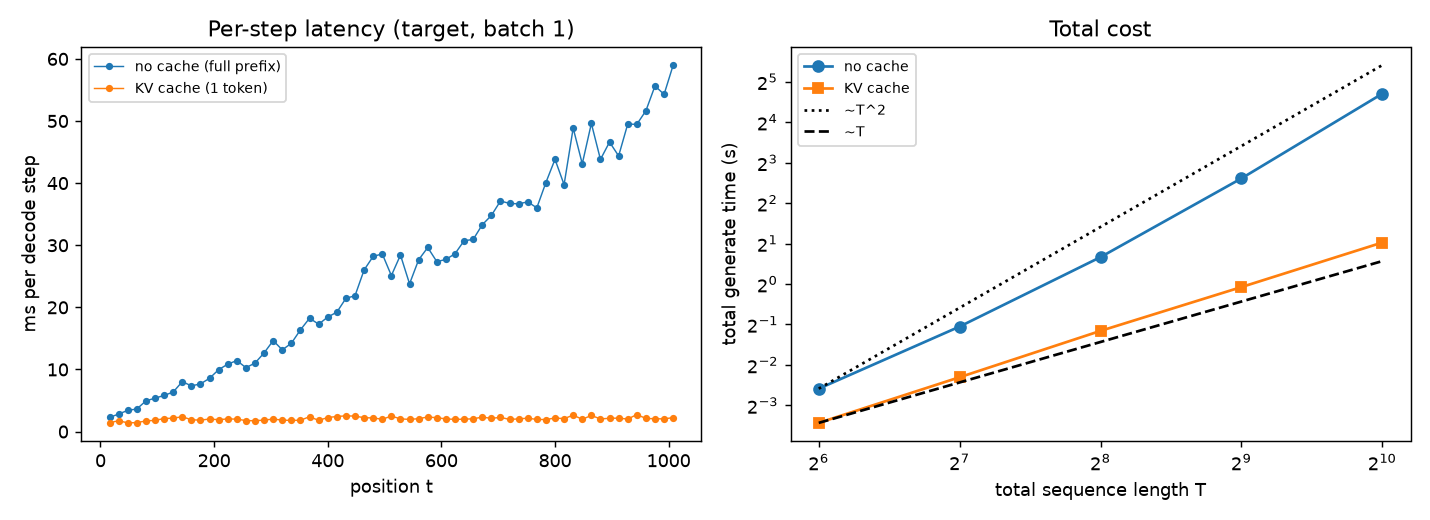
\includegraphics[width=\linewidth]{kv_cache_timing.png}
\caption{CPU：单步延迟（左）与总生成时间（右，log-log，虚线为 $T$ 与 $T^2$ 斜率）。}\label{fig:cpu-kv}
\end{figure}

\Cref{fig:cpu-spec} 是 CPU 推测解码：左图测得的「每次 target 调用产出的 token 数」与 $(1-\alpha^{\gamma+1})/(1-\alpha)$ 的差在 4\% 以内（贪心 $\gamma{=}8$ 时 8.24 对 8.56，
差距来自每个 prompt 最后一轮被截短的 $\gamma$）；右图是实测加速，只有 0.98--1.99 倍，明显低于「验证免费」的预测。原因是 CPU 上验证 $\gamma{+}1$ 个 token 的 forward 要花单 token 的
1.41--1.61 倍（\texttt{speculative.csv} 的 \texttt{verify\_cost\_vs\_1tok}），而 $c{=}0.256$ 被 Python 调用开销抬高（参数量之比只有 0.04）。

\begin{figure}[H]
\centering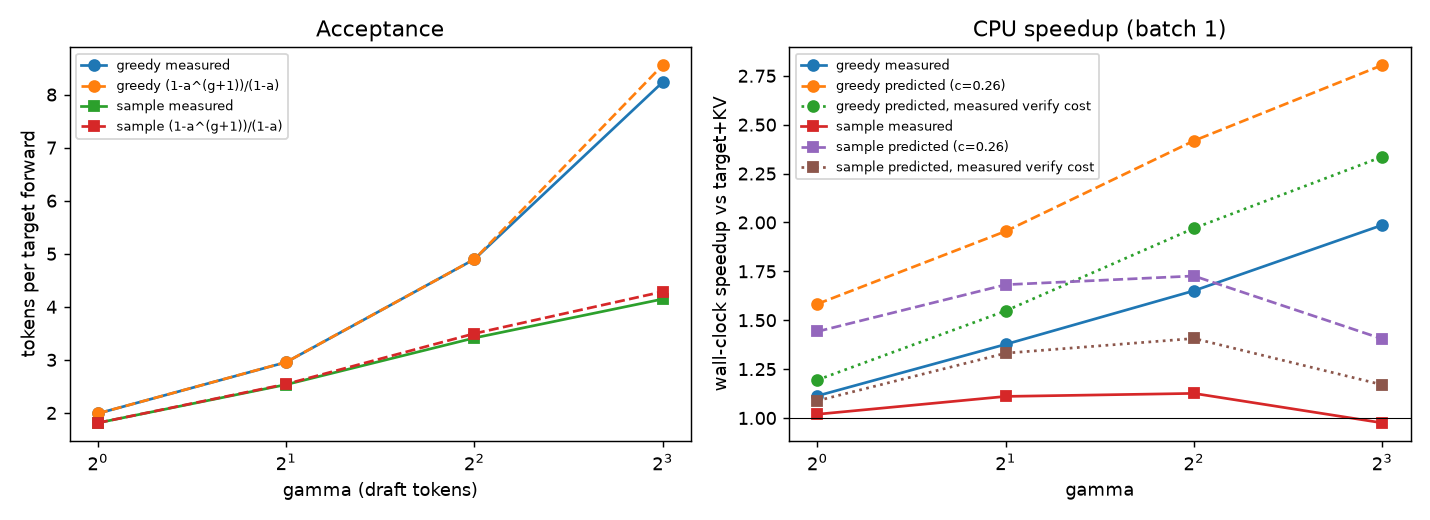
\includegraphics[width=\linewidth]{speculative.png}
\caption{CPU：每次 target forward 产出的 token 数（左）与 wall-clock 加速（右）。}\label{fig:cpu-spec}
\end{figure}

\begin{findingbox}[：CPU 原型]
CPU 上 KV cache 的收益来自省掉 $O(T)$ 倍的线性层计算（T=1024 时 12.82 倍）；推测解码的「token 数公式」很准，但加速被两件事吃掉：验证不免费（$v\approx1.4$--$1.6$）和 $c$ 被调用开销抬高。
这两点在 GPU 上会怎样变化，是 GPU 实验要回答的问题。
\end{findingbox}

\subsection{GPU 正确性：与 HF 对齐，贪心输出一致}

\Cref{tab:parity} 与 \cref{fig:parity} 给出 fp32（关闭 TF32）下我们的 forward 与 HF \texttt{GPT2LMHeadModel}（eager attention）在 2 条 $\times$ 128 token 的
WikiText 输入上的 logits 差。gpt2-large / gpt2-xl 的最大绝对误差为 $4.2\times10^{-5}$ / $4.6\times10^{-5}$，满足 $\sim10^{-4}$ 的要求；
gpt2 与 gpt2-medium 的绝对误差更大（$2.26\times10^{-3}$ / $4.58\times10^{-4}$），这是因为这两个模型的 logits 本身很大（最大 $|$logit$|$ 282.2 / 348.4），
相对误差仅 $8.0\times10^{-6}$ / $1.3\times10^{-6}$，softmax 概率的最大差 $\le 9.5\times10^{-6}$，argmax 一致率都是 1.0。KV cache 路径（64 token prefill + 64 次单 token decode）
与 HF 的差在同一量级。

\begin{table}[H]
\centering\small
\caption{fp32 logits 对 HF transformers 5.21.0（\texttt{verify.jsonl}）}\label{tab:parity}
\begin{tabular}{lrrrrrr}
\toprule
模型 & 无 cache 最大 $|\Delta|$ & KV 最大 $|\Delta|$ & 平均 $|\Delta|$ & 最大 $|$logit$|$ & 相对误差 & 最大 $|\Delta p|$ \\
\midrule
gpt2 & 2.26e-3 & 1.48e-3 & 7.2e-5 & 282.2 & 8.0e-6 & 9.5e-6 \\
gpt2-medium & 4.58e-4 & 1.04e-3 & 4.1e-5 & 348.4 & 1.3e-6 & 5.6e-6 \\
gpt2-large & 4.20e-5 & 4.58e-5 & 1.5e-6 & 48.6 & 8.6e-7 & 2.8e-6 \\
gpt2-xl & 4.58e-5 & 3.81e-5 & 2.0e-6 & 50.9 & 9.0e-7 & 2.2e-6 \\
\bottomrule
\end{tabular}
\end{table}

\begin{figure}[H]
\centering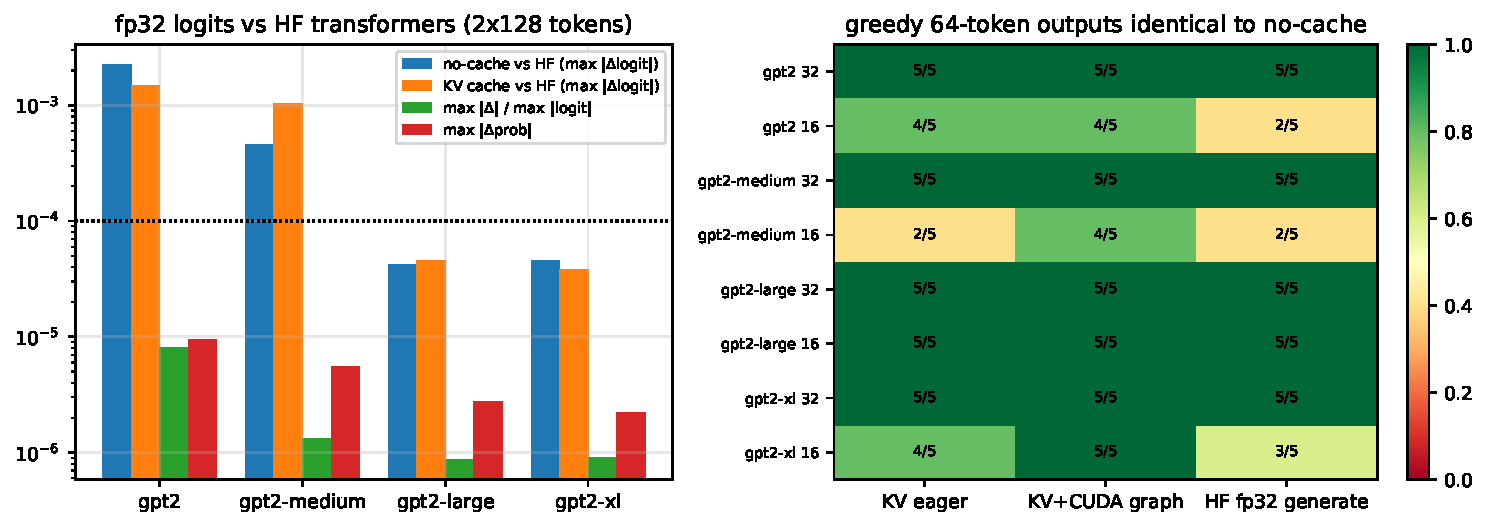
\includegraphics[width=\linewidth]{gpu_parity.pdf}
\caption{左：fp32 logits 误差（log 轴，虚线 $10^{-4}$）；右：5 个 prompt $\times$ 64 个新 token 的贪心输出与无 cache 版本完全相同的比例，按模型与精度分行。}\label{fig:parity}
\end{figure}

贪心一致性：fp32 下 4 个模型 $\times$ 5 个 prompt，KV eager、KV + CUDA Graph、HF \texttt{generate} 三者的 64 个新 token 与无 cache 版本\textbf{全部逐 token 相同}（60/60）。
fp16 下出现分叉：例如 gpt2-medium 的 KV eager 只有 2/5 与无 cache 相同。这不是 bug，而是 fp16 下不同形状的 GEMM（整段 prefill 对单 token）累加顺序不同，
在 top-2 logit 几乎相等的位置翻转 argmax；之后序列自然分叉。推测解码实验里我们直接测了分叉点的 top-2 差（\cref{sec:spec-res}），全部 $\le 0.0078$，正好是 fp16 在这个量级上的 1 个 ulp。

\begin{findingbox}[：正确性]
「贪心输出必须一致」只能在 fp32 下当作硬约束检查（本实验 60/60 通过，推测解码 fp32 120/120 通过）；fp16 下应改为「分叉只发生在 top-2 差 $\le$ 1 ulp 的平局处」。
面试时把这两种判据分清楚，比声称 fp16 也 bit-exact 更可信。
\end{findingbox}

\subsection{每 token 延迟 vs 上下文长度与模型大小}\label{sec:lat}

\Cref{fig:lat} 左图是 batch 1、fp16 下三种实现的每 token 延迟。几个出乎直觉的现象：
\begin{enumerate}
  \item \textbf{短上下文时 KV eager 比无 cache 还慢}。gpt2-xl 在上下文 16 时无 cache 4.84 ms、KV eager 6.21 ms；直到上下文 128 两者才持平（6.71 对 6.16 ms）。
        原因是 eager 模式每层要多发 cache 写入、切片、mask 等小 kernel，batch 1 时 GPU 大部分时间在等 CPU 发 kernel（launch-bound），省下的 FLOP 根本不在关键路径上。
  \item \textbf{无 cache 的代价在长上下文才显现}：gpt2-xl 上下文 1024 时无 cache 每 token 20.62 ms，KV eager 6.32 ms，KV + CUDA Graph（bmm attention）4.22 ms，后者是前者的 4.9 倍。
  \item \textbf{CUDA Graph 消掉了 launch 开销}：gpt2-xl 上下文 16 时从 6.21 ms（eager）降到 3.74 ms（graph），gpt2 从 1.56 ms 降到 0.49 ms（\texttt{latency.jsonl}）。
  \item \textbf{SDPA + bool mask 的 decode attention 随上下文明显变慢}：gpt2-xl 从上下文 16 的 3.74 ms 涨到 1024 的 6.36 ms，而 roofline 预测只涨 0.20 ms（KV 读取量 315 MB / 1.52 TB/s）。
        batch 1 时 attention 只有 $B\times H = 25$ 个 (batch, head) 对，SDPA 的 memory-efficient kernel 按它们分 block，170 个 SM 大多空闲。改成显式 $QK^\top$/softmax/$PV$
        （cuBLAS 会沿 $T$ 维切分）后，gpt2-xl 上下文 1024 时降到 4.22 ms，曲线几乎变平。这正是 Flash-Decoding~\cite{flashdec}（split-KV）要解决的问题。
\end{enumerate}

\begin{figure}[H]
\centering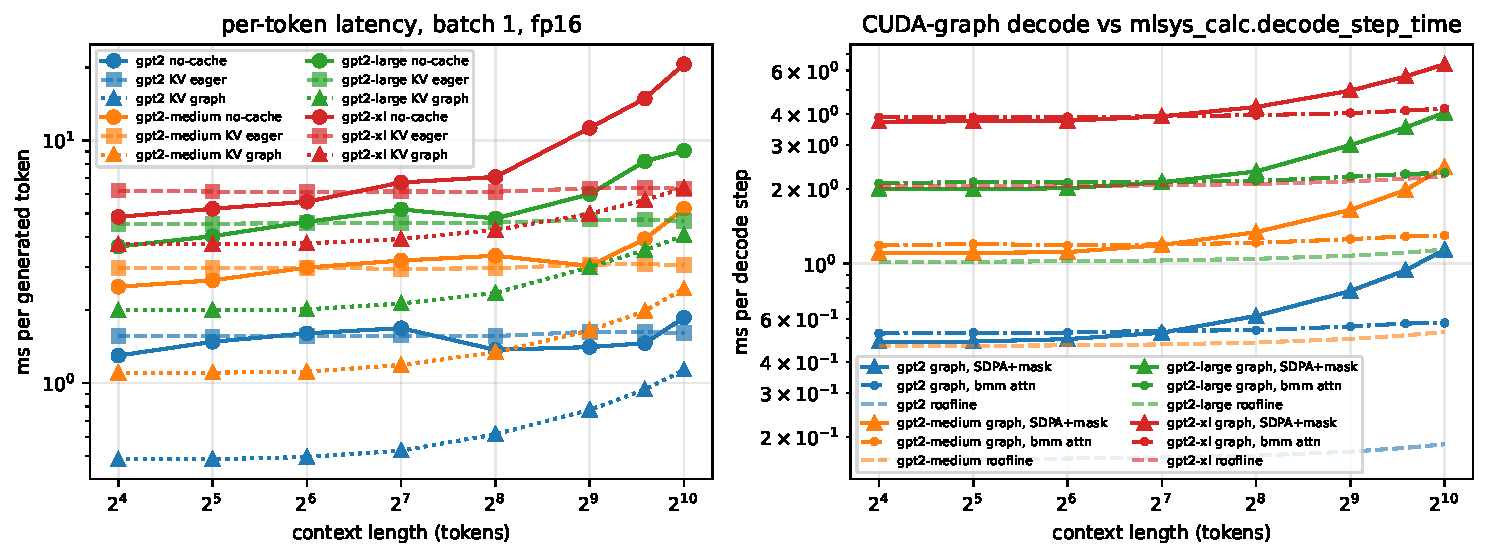
\includegraphics[width=\linewidth]{gpu_latency_vs_ctx.pdf}
\caption{左：三种实现的每 token 延迟（log-log）；右：CUDA Graph decode（SDPA+mask 与 bmm 两种 attention）对比 \texttt{mlsys\_calc.decode\_step\_time} 的 roofline 下界（虚线）。}\label{fig:lat}
\end{figure}

\Cref{fig:lat-model} 把上下文 128 时的延迟画成权重字节数的函数。CUDA Graph 的延迟几乎是权重字节数的线性函数，但斜率约是「权重 / 带宽」虚线的 2 倍：
gpt2-xl 3.92 ms 对 roofline 2.07 ms。\Cref{fig:overhead} 把差值（实测 $-$ roofline）对层数作图：gpt2-large 与 gpt2-xl 每层多出 30.4--38.6 µs，与层数近似成正比，
相当于每层约 14 个 kernel、每个 kernel 2--3 µs 的固定开销（kernel 启动、尾部 wave 与依赖等待即使在 graph 里也存在）。加入 bmm attention 后在 4 个模型、3 个上下文长度（16 / 128 / 1024）上重新拟合，每层开销都落在 29.9--41.0 µs（直线拟合的斜率为 40.0--42.9 µs/层，\texttt{decode\_overhead.csv}），与上下文长度基本无关。

\begin{figure}[H]
\centering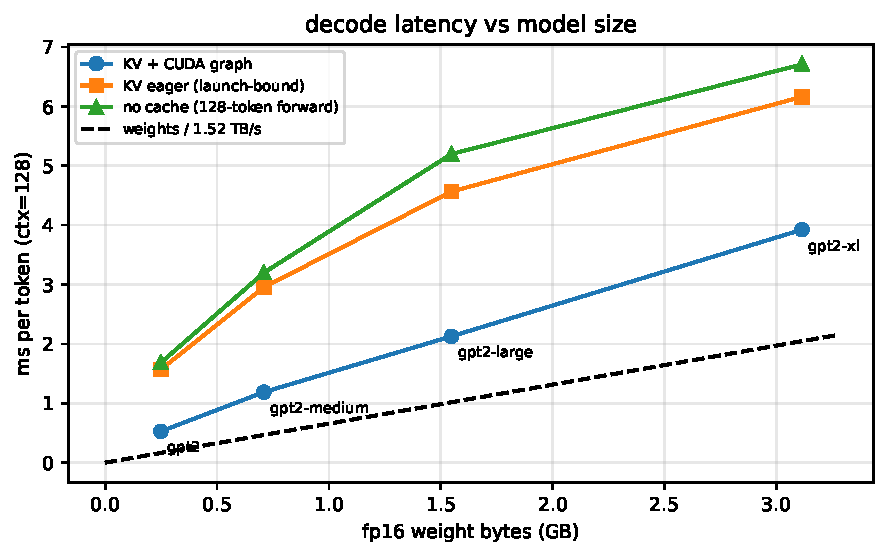
\includegraphics[width=0.62\linewidth]{gpu_latency_vs_model.pdf}
\caption{上下文 128 时每 token 延迟 vs fp16 权重字节数；黑色虚线为「权重 / 实测带宽」。}\label{fig:lat-model}
\end{figure}

\begin{figure}[H]
\centering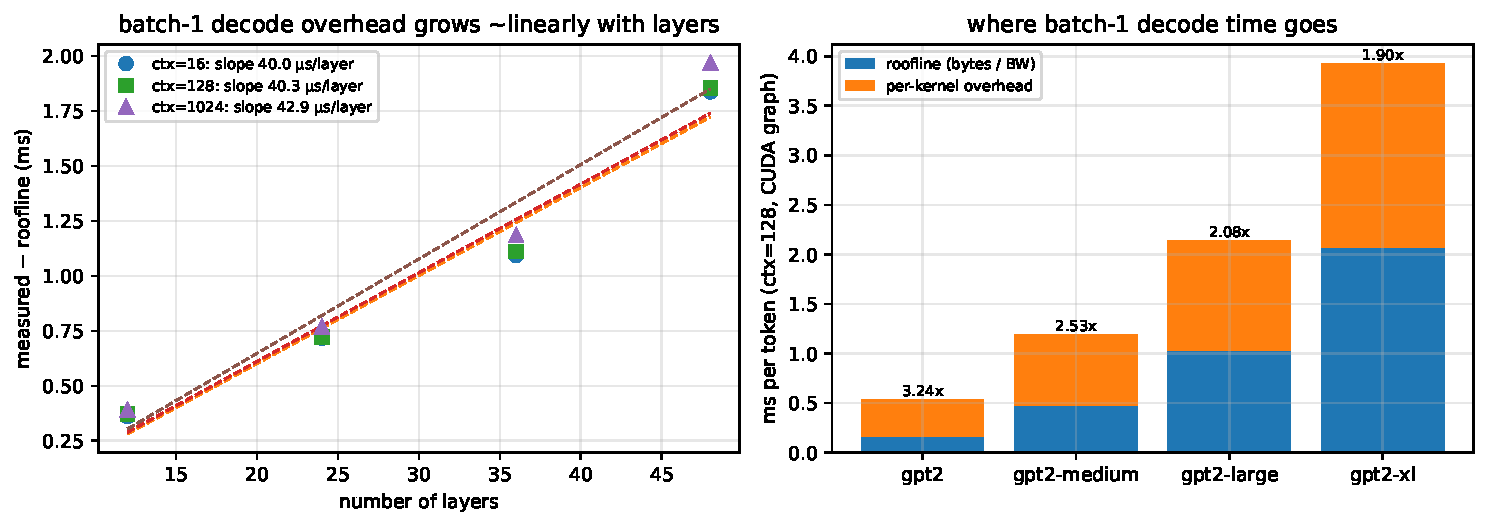
\includegraphics[width=\linewidth]{gpu_decode_overhead.pdf}
\caption{左：batch 1 decode 的「实测 $-$ roofline」随层数线性增长（三个上下文长度各拟合一条直线）；右：上下文 128 时延迟拆成 roofline 部分与固定开销部分，柱顶标注实测/预测比。}\label{fig:overhead}
\end{figure}

\begin{findingbox}[：batch 1 decode 的时间去哪了]
在 RTX 5090 上，gpt2-xl batch 1 decode 只达到实测带宽的约一半（实测/roofline = 1.90）；剩下的一半是与层数成正比的 per-kernel 固定开销。
模型越小，这个比例越大（gpt2 是 3.24 倍）。这就是为什么推测解码里小 draft 的 $c$ 远大于参数量之比，也是 kernel fusion / 更少 kernel 的价值所在。
\end{findingbox}

\subsection{Prefill 与 decode}

\Cref{fig:prefill} 是生成 128 个新 token 时 prefill 与 decode 的时间拆分。prefill 一次处理整个 prompt，属于 compute 友好的大 GEMM：
gpt2-xl 处理 512 个 prompt token 的 prefill 只要 12.80 ms，而之后 127 个 decode token 要 680.0 ms（CUDA Graph）——每个 token 的 decode 代价约是 prefill 中每个 token 的 214 倍。
无 cache 版本的 decode 时间随 prompt 变长而增长（gpt2-xl P=128 时 853.4 ms、P=512 时 1627.8 ms），KV 版本基本不变（782.8 / 796.5 ms，eager）。
注意 CUDA Graph 版本在 P=896 时（810.5 ms）反而比 eager（794.6 ms）慢：\texttt{generate\_graph} 的 attention 固定在整个 $T_{\max}=1024$ 缓冲区上用 SDPA+mask，
这把 \cref{sec:lat} 里 SDPA 的长上下文问题放大了。

\begin{figure}[H]
\centering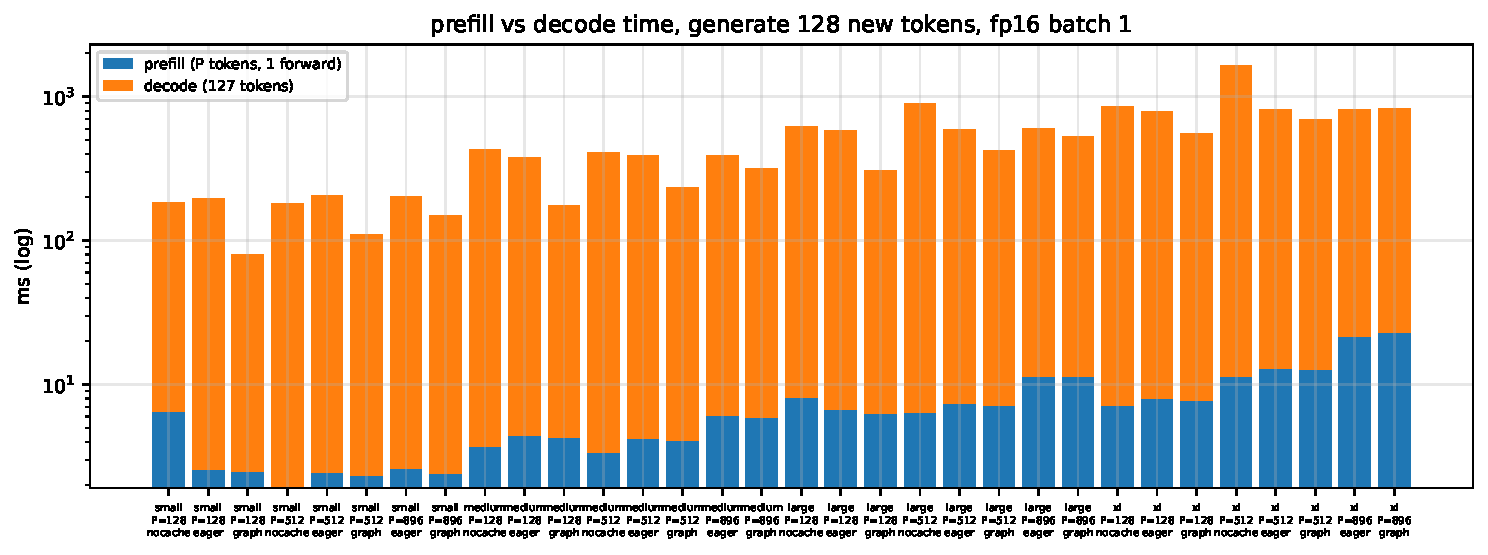
\includegraphics[width=\linewidth]{gpu_prefill_decode.pdf}
\caption{prefill（下）与 decode 127 个 token（上）的时间，log 轴；横轴为 模型 / prompt 长度 / 实现。}\label{fig:prefill}
\end{figure}

\subsection{吞吐 vs batch：memory-bound 到 compute-bound 的拐点}

\Cref{fig:batch} 是 CUDA Graph decode 的 tokens/s 随 batch 的变化（实线），虚线是 \path{mlsys_calc.decode_step_time} 用实测峰值（1522 GB/s、223.4 TFLOP/s）给出的上界。
上下文 256 时，gpt2-xl 的步时间从 batch 1 的 4.27 ms 到 batch 16 的 5.27 ms 几乎不变（权重读一次，被 16 个序列共享），吞吐近似线性增长到 3{,}039 tok/s；
此后 KV 读取量随 batch 线性增长，batch 256 时 KV 达到 20.1 GB（权重只有 3.1 GB），步时间 20.0 ms，吞吐 12{,}801 tok/s，仍然是 memory-bound——
在上下文 256 下，GPT-2 的 decode 永远到不了 compute roof，因为强度被 KV 封顶。\par 为了看到 weights-only 的拐点，又在上下文 32 下重复了 batch 扫描（\texttt{ctx32/batch.jsonl}），此时 KV 很小，强度近似等于 $B$。
gpt2-xl 的步时间在 $B{=}2$--16 时几乎不变（4.14--4.28 ms），吞吐从 $B{=}1$ 的 268.7 tok/s 涨到 $B{=}16$ 的 3{,}739 tok/s（13.9 倍）；
$B{=}32$ 起步时间开始上升（5.44 ms），从 $B{=}16$ 到 256（batch 再翻 16 倍）吞吐只再涨 6.95 倍，到 25{,}999 tok/s。$B{=}256$ 时强度 142 FLOP/B，已接近 ridge（147），
实测 $2NB/t$ = 80.9 TFLOP/s，是 GEMM 实测峰值的 36\%。也就是说，实测拐点（$B\approx16$--32）比 roofline 拐点（$B\approx147$）早得多：小 $M$ 的 GEMM 达不到峰值，
$B$ 一过 16 步时间就开始随 $B$ 增长。

\begin{figure}[H]
\centering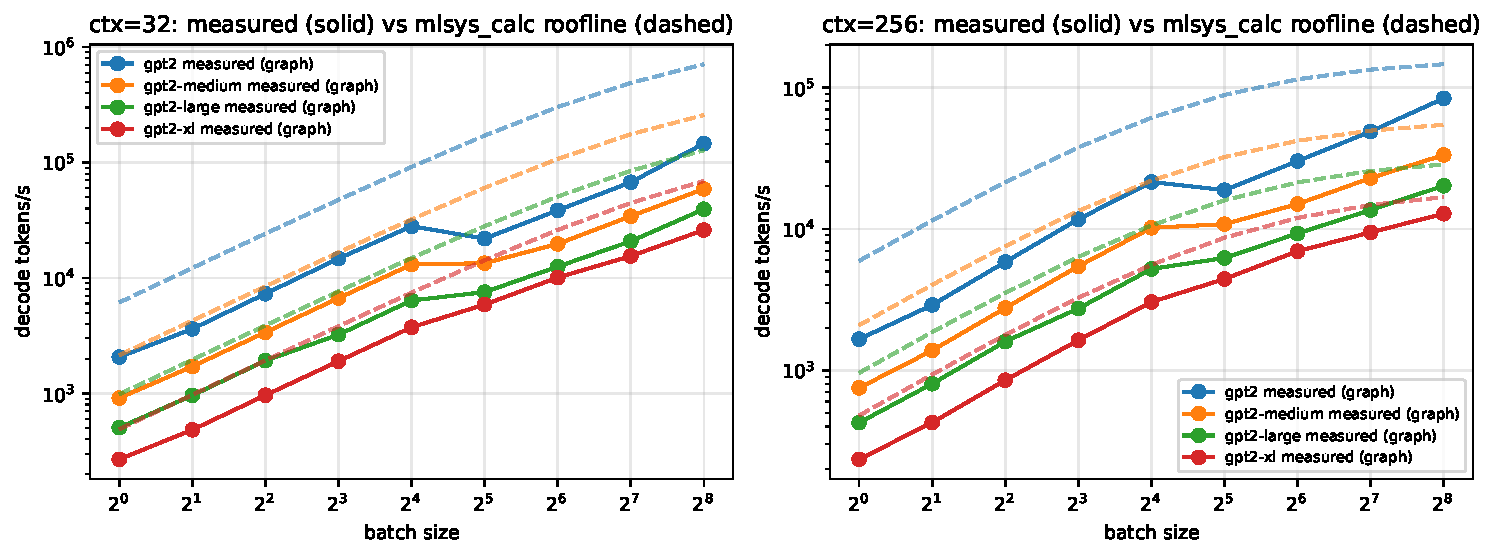
\includegraphics[width=\linewidth]{gpu_batch_throughput.pdf}
\caption{decode 吞吐 vs batch（log-log），实线为实测（CUDA Graph），虚线为 roofline 预测。}\label{fig:batch}
\end{figure}

\begin{figure}[H]
\centering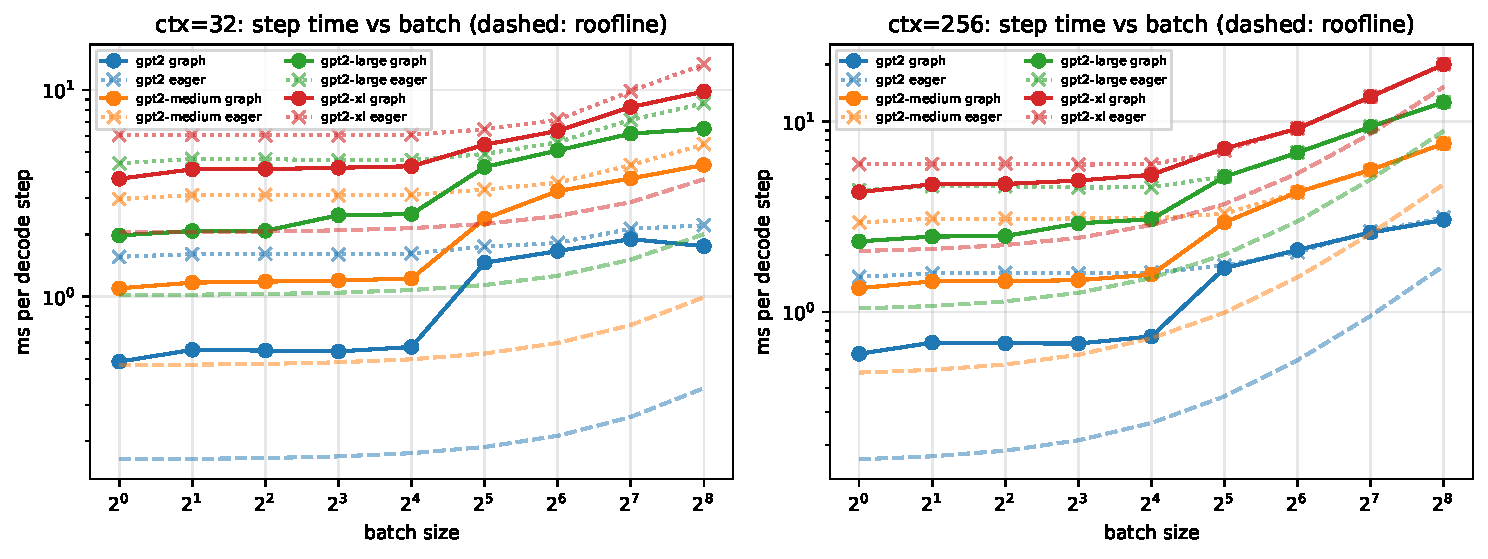
\includegraphics[width=\linewidth]{gpu_batch_steptime.pdf}
\caption{每步时间 vs batch：graph（实线）、eager（点线）、roofline（虚线）。小 batch 时 eager 与 graph 差一个固定的 launch 开销，大 batch 时两者重合。}\label{fig:steptime}
\end{figure}

\begin{figure}[H]
\centering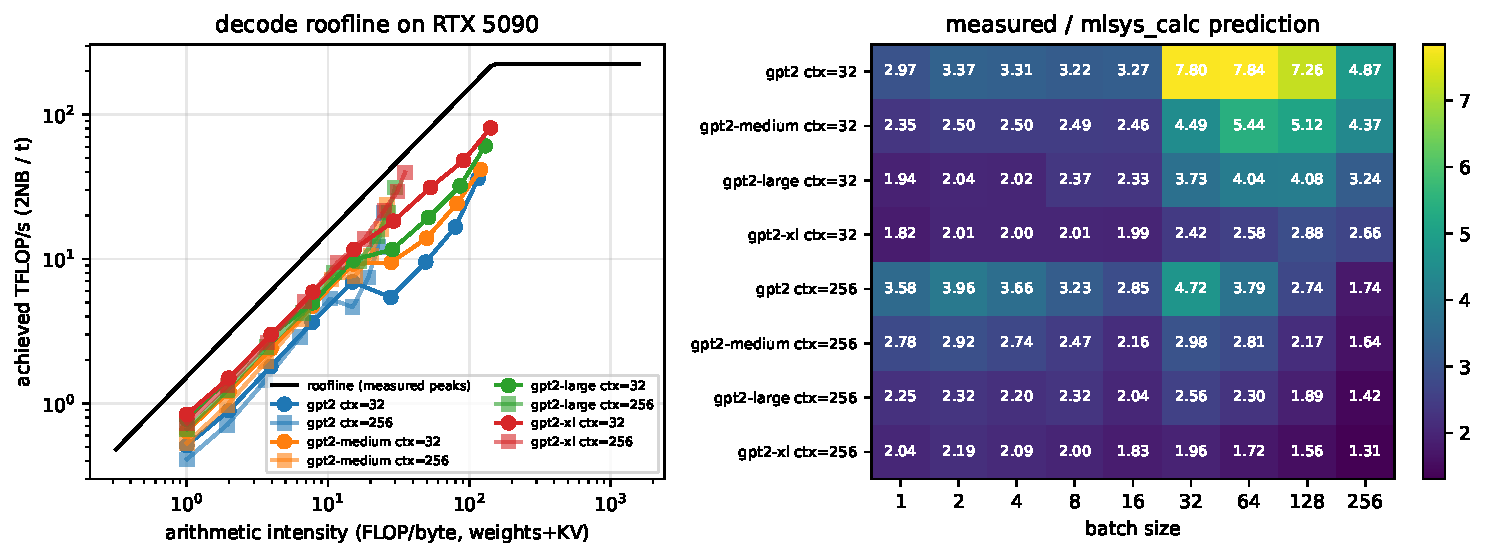
\includegraphics[width=\linewidth]{gpu_roofline_ratio.pdf}
\caption{左：roofline 图，横轴为 \texttt{decode\_step\_time} 给出的强度（FLOP / 权重+KV 字节），纵轴为实测 $2NB/t$；右：实测 / 预测时间之比。}\label{fig:roof}
\end{figure}

\Cref{fig:roof} 右图的比值是本节最重要的「模型 vs 实测」结论：上下文 256 下，gpt2-large / gpt2-xl 的实测 / 预测比在 1.31--2.56 之间，随 batch 增大而下降（xl：$B{=}1$ 为 2.04，$B{=}256$ 为 1.31），因为固定开销被摊薄、KV 读取占比上升；
gpt2 / gpt2-medium 在 1.64--4.72 之间，小模型的 per-kernel 开销占比更大。上下文 32 下比值更高（xl 1.82--2.89，gpt2 2.97--7.84），因为这时预测时间更短、
而实测在 $B\ge32$ 后就被 GEMM 效率拖慢。总的来说，\texttt{decode\_step\_time} 在这台机器上是一个可靠的\emph{下界}，大模型、大 batch 时偏差在 1.3--2 倍，
小模型或短上下文时可以差到 3--8 倍，不能直接当作延迟预测。

\subsection{KV cache 显存：实测 vs 公式}

\Cref{fig:mem} 对 4 个模型、$T\in\{128,256,512,1024\}$、$B\in\{1,8,32,64\}$ 共 63 个组合（超过 16 GB 的跳过），比较 \texttt{torch.cuda.memory\_allocated}
在分配 \texttt{StaticKV} 前后的差与公式 $2\cdot L\cdot B\cdot H\cdot d_h\cdot T\cdot 2$ 字节（等于 \texttt{mlsys\_calc.kv\_cache\_bytes}）。58/63 个组合\textbf{逐字节相等}；
其余 5 个都是 batch 1 的小缓冲区，被 PyTorch caching allocator 向上取整（例如 gpt2-large $T{=}128$：公式 23{,}592{,}960 B，实测 25{,}165{,}824 B = 24 MiB），
最大偏差是 gpt2 $T{=}128,B{=}1$ 的 1.39 倍（4.72 MB 对 6.55 MB）。decode 一步的额外峰值（激活 + workspace）只有 1.1--9.6 MB，与 KV 相比可以忽略。
gpt2-xl 每 token 的 KV 是 $2\times48\times1600\times2 = 307{,}200$ 字节（300 KiB），$T{=}1024, B{=}32$ 时 10.07 GB，已是权重（3.12 GB）的 3.2 倍。

\begin{figure}[H]
\centering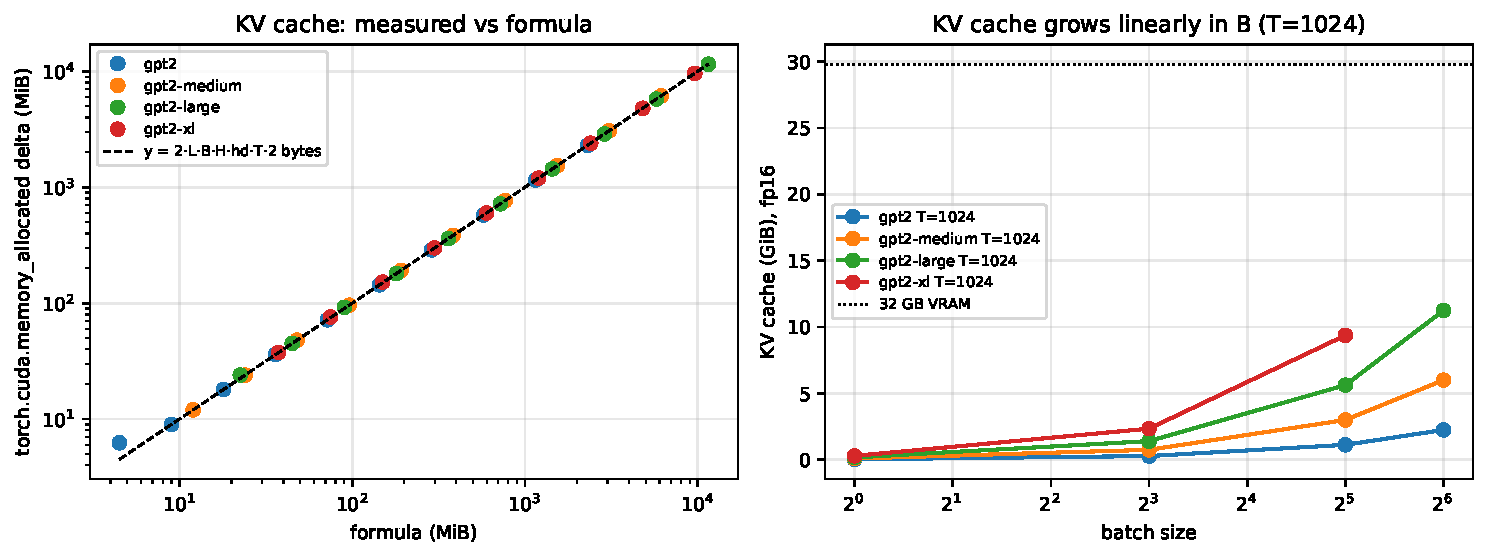
\includegraphics[width=\linewidth]{gpu_kv_memory.pdf}
\caption{左：实测 KV 分配 vs 公式（虚线 $y=x$）；右：$T{=}1024$ 时 KV 随 batch 线性增长（点线为 32 GB 显存）。}\label{fig:mem}
\end{figure}

\subsection{推测解码：接受率与每次 target 调用的 token 数}\label{sec:spec-res}

主实验：draft = gpt2（124M），target = gpt2-large（774M）和 gpt2-xl（1.5B），100 个 WikiText prompt（每个 64 token），每个生成 64 个新 token，
$\gamma\in\{1,\dots,8\}$，温度 $T\in\{0, 0.7, 1.0\}$，全部用 CUDA Graph、fp16。

\Cref{fig:alpha} 显示 $\hat\alpha$ 基本不随 $\gamma$ 变化：gpt2→gpt2-large 贪心约 0.74--0.76，$T{=}1$ 约 0.66--0.68；gpt2→gpt2-xl 贪心 0.70--0.72，$T{=}1$ 0.63--0.65。
采样模式下 $\hat\alpha$ 与 $\mathbb{E}[\sum_x\min(p,q)]$ 吻合到小数点后两位（例如 gpt2-xl $\gamma{=}4,T{=}1$：0.6285 对 0.6423；gpt2-large $\gamma{=}8,T{=}1$：0.6629 对 0.6644）。
而错误定义 accepted/proposed 随 $\gamma$ 单调下降，到 $\gamma{=}8$ 只剩 0.21--0.34，用它代入公式会严重低估。

\begin{figure}[H]
\centering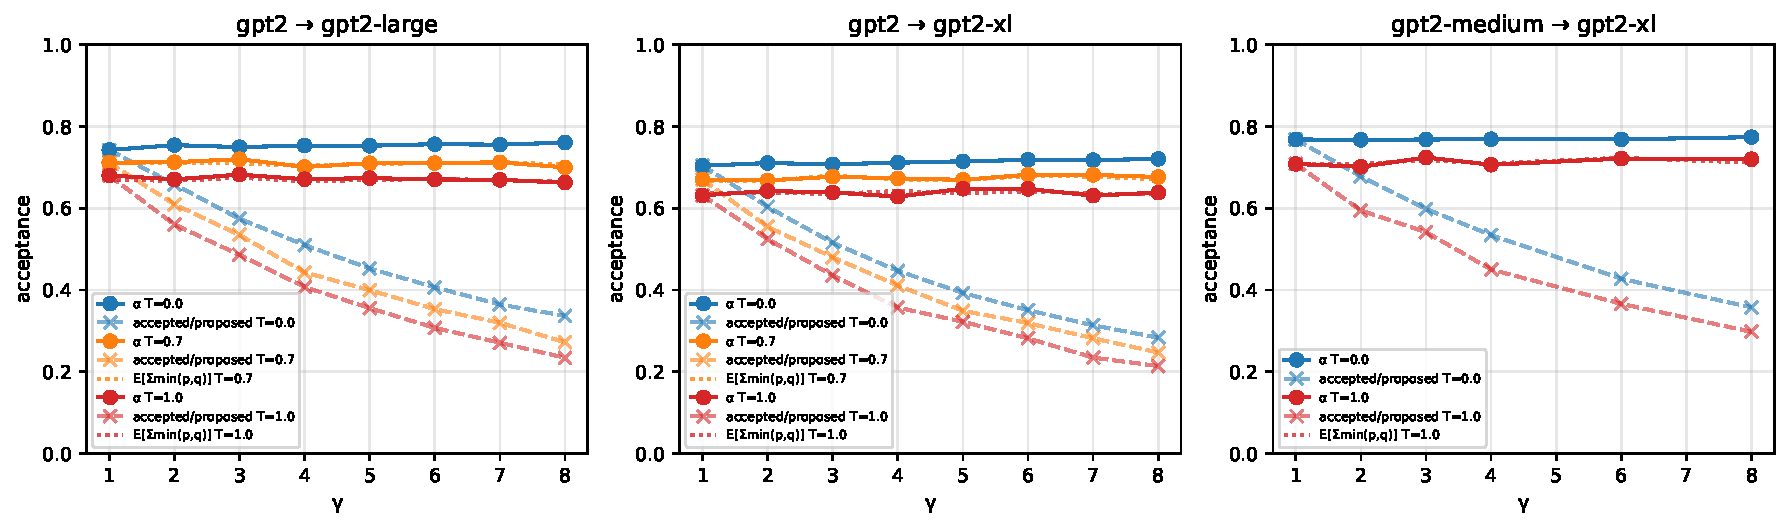
\includegraphics[width=\linewidth]{gpu_spec_alpha.pdf}
\caption{接受率：正确的 $\hat\alpha$（实线）、错误的 accepted/proposed（叉号虚线）、$1-\mathrm{TV}$ 的期望（点线，仅采样）。}\label{fig:alpha}
\end{figure}

\Cref{fig:tokens} 是每次 target forward 产出的 token 数。实测值与 $(1-\hat\alpha^{\gamma+1})/(1-\hat\alpha)$ 在采样模式下几乎重合（gpt2-xl $\gamma{=}8,T{=}1$：2.713 对 2.716），
贪心模式下 $\gamma$ 大时实测略低（gpt2-xl $\gamma{=}8$：3.268 对 3.392）。\Cref{fig:hist} 解释了原因：贪心时每轮接受数的分布比截断几何分布「两头更重」——
0 个接受和全部接受都偏多（gpt2-large $\gamma{=}8$ 全接受的比例约 0.15，几何分布预测约 0.11）。即接受事件不是 i.i.d.：有的上下文 draft 几乎总对（套话、专有名词的后半），有的几乎总错。
$\alpha$ 的异质性让 $\mathbb{E}[\alpha^{k}] \ne \bar\alpha^{k}$，公式基于平均 $\alpha$，所以在长 $\gamma$ 时有偏。

\begin{figure}[H]
\centering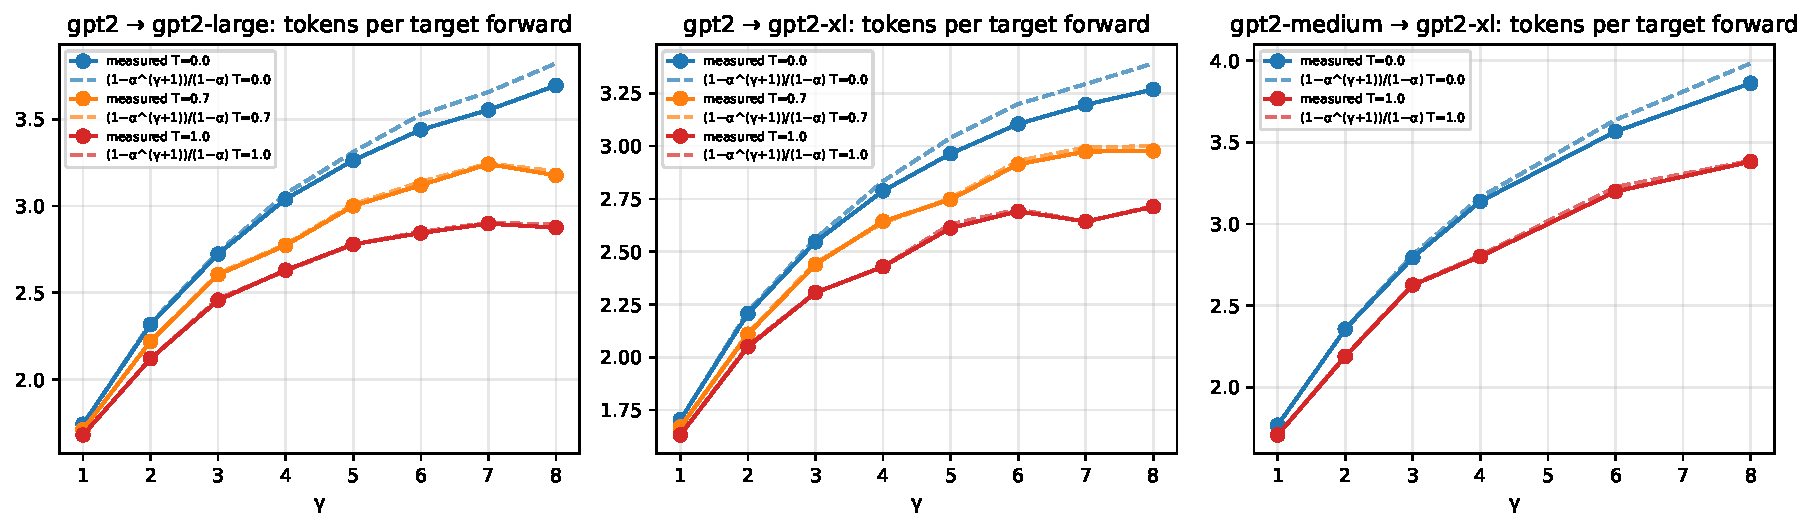
\includegraphics[width=\linewidth]{gpu_spec_tokens.pdf}
\caption{每次 target forward 的 token 数：实测（实线）vs 公式（虚线）。}\label{fig:tokens}
\end{figure}

\begin{figure}[H]
\centering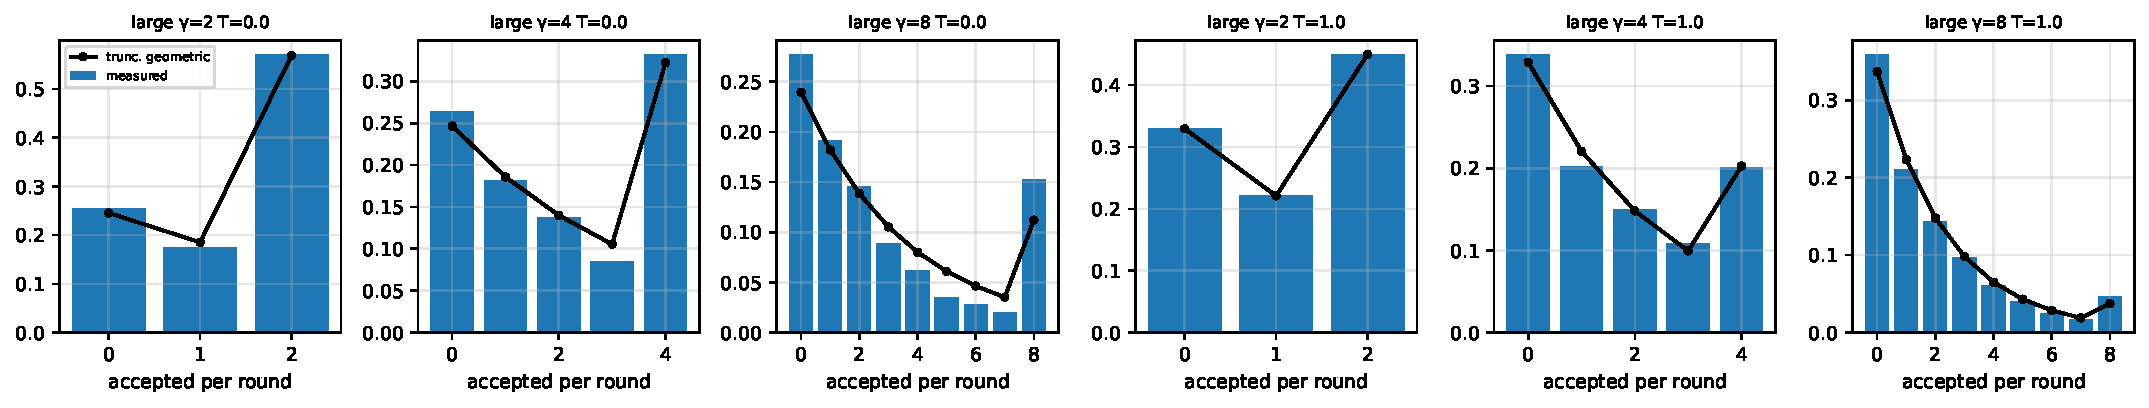
\includegraphics[width=\linewidth]{gpu_spec_accept_hist.pdf}
\caption{每轮接受数的分布（gpt2→gpt2-large）vs 用 $\hat\alpha$ 计算的截断几何分布（黑线）。}\label{fig:hist}
\end{figure}

\textbf{贪心精确性}：fp32 下（gpt2→gpt2-xl，20 个 prompt $\times$ 64 token，$\gamma\in\{1,4,8\}$，eager 与 CUDA Graph 两种实现）推测解码输出与 target 单独贪心解码\textbf{120/120 完全一致}（\texttt{spec\_exact.jsonl}）。
fp16 主实验中 gpt2-large 94/100、gpt2-xl 91/100 一致，不一致的 prompt 在所有 $\gamma$ 下都是同一批，且分叉点 target 的 top-2 logit 差最大只有 0.0078125（多数为 0），即 fp16 平局。

\subsection{推测解码：wall-clock 加速}

\Cref{tab:spec} 摘录主要结果，完整数据见 \texttt{spec\_summary.csv}。基线是同一套 CUDA Graph 的 target 单独 decode：gpt2-large 429.3 tok/s、gpt2-xl 223.9 tok/s（贪心）。
实测 $c = t_{\text{draft}}/t_{\text{target}}$：gpt2-large 0.253、gpt2-xl 0.138（draft 单步 0.56 ms；参数量之比分别是 0.16 和 0.08，同样被 per-kernel 开销抬高）。
验证代价 $v$：gpt2-xl 在 $\gamma{=}1$--8 时只有 1.10--1.12（验证 9 个 token 只比 1 个 token 贵 12\%，这才是 GPU 上推测解码成立的根本原因）；gpt2-large 在 $\gamma\le3$ 时 1.07，$\gamma\ge4$ 跳到 1.24。

\begin{table}[H]
\centering\small
\caption{推测解码主要结果（100 prompt $\times$ 64 token，fp16，CUDA Graph；\texttt{spec\_summary.csv}）}\label{tab:spec}
\begin{tabular}{llrrrrrrrr}
\toprule
target & $T$ & $\gamma$ & $\hat\alpha$ & tok/调用 & 公式 & $c$ & $v$ & 预测 $E/(\gamma c+v)$ & 实测加速 \\
\midrule
gpt2-large & 0 & 3 & 0.750 & 2.723 & 2.733 & 0.253 & 1.070 & 1.494 & \textbf{1.348} \\
gpt2-large & 1.0 & 3 & 0.682 & 2.457 & 2.465 & 0.253 & 1.070 & 1.348 & 1.177 \\
gpt2-large & 1.0 & 5 & 0.674 & 2.779 & 2.778 & 0.253 & 1.242 & 1.108 & 0.986 \\
gpt2-large & 1.0 & 8 & 0.663 & 2.875 & 2.893 & 0.253 & 1.247 & 0.884 & 0.794 \\
gpt2-xl & 0 & 3 & 0.708 & 2.547 & 2.562 & 0.137 & 1.106 & 1.688 & \textbf{1.631} \\
gpt2-xl & 0 & 4 & 0.712 & 2.788 & 2.834 & 0.138 & 1.115 & 1.701 & 1.629 \\
gpt2-xl & 0.7 & 3 & 0.677 & 2.440 & 2.447 & 0.137 & 1.106 & 1.612 & 1.528 \\
gpt2-xl & 1.0 & 3 & 0.639 & 2.306 & 2.307 & 0.137 & 1.106 & 1.520 & 1.454 \\
gpt2-xl & 1.0 & 8 & 0.638 & 2.713 & 2.716 & 0.138 & 1.118 & 1.224 & 1.165 \\
\bottomrule
\end{tabular}
\end{table}

\begin{figure}[H]
\centering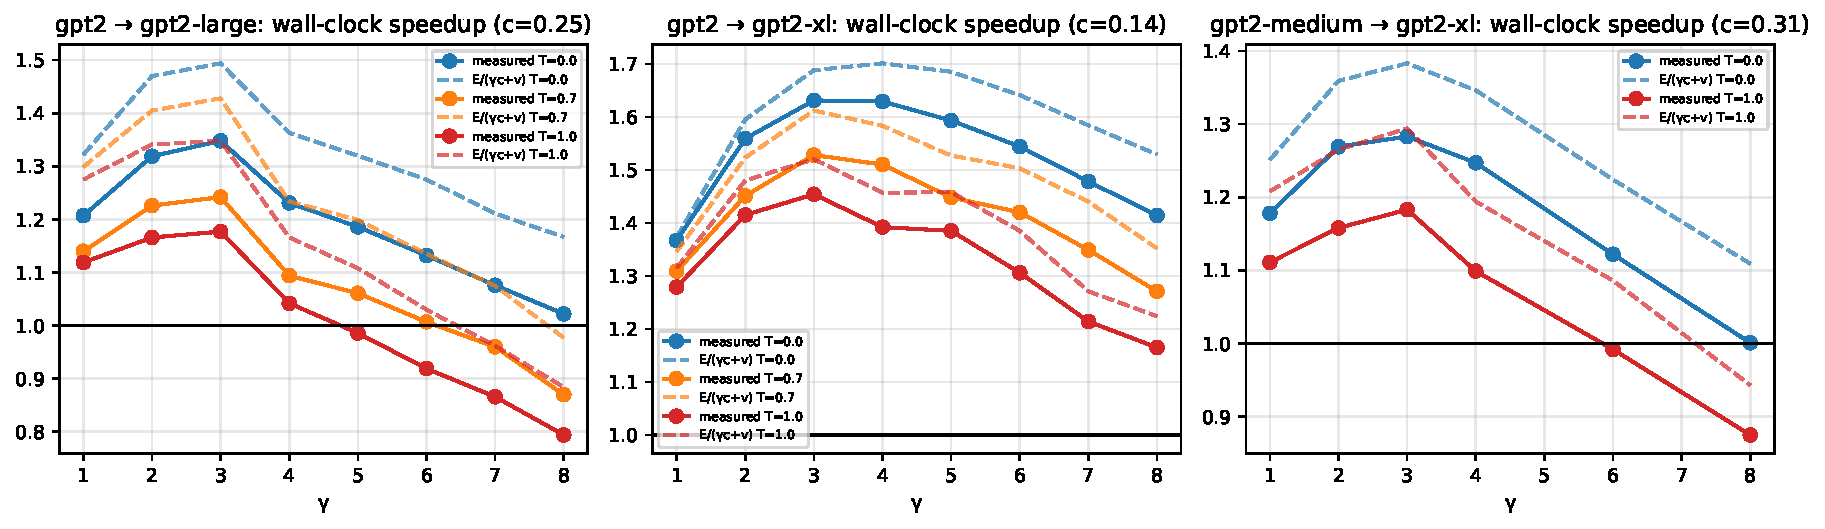
\includegraphics[width=\linewidth]{gpu_spec_speedup.pdf}
\caption{wall-clock 加速 vs $\gamma$：实测（实线）vs 用实测 $c$、$v$、$\hat\alpha$ 代入 \cref{eq:spec}（虚线）。}\label{fig:speedup}
\end{figure}

\begin{figure}[H]
\centering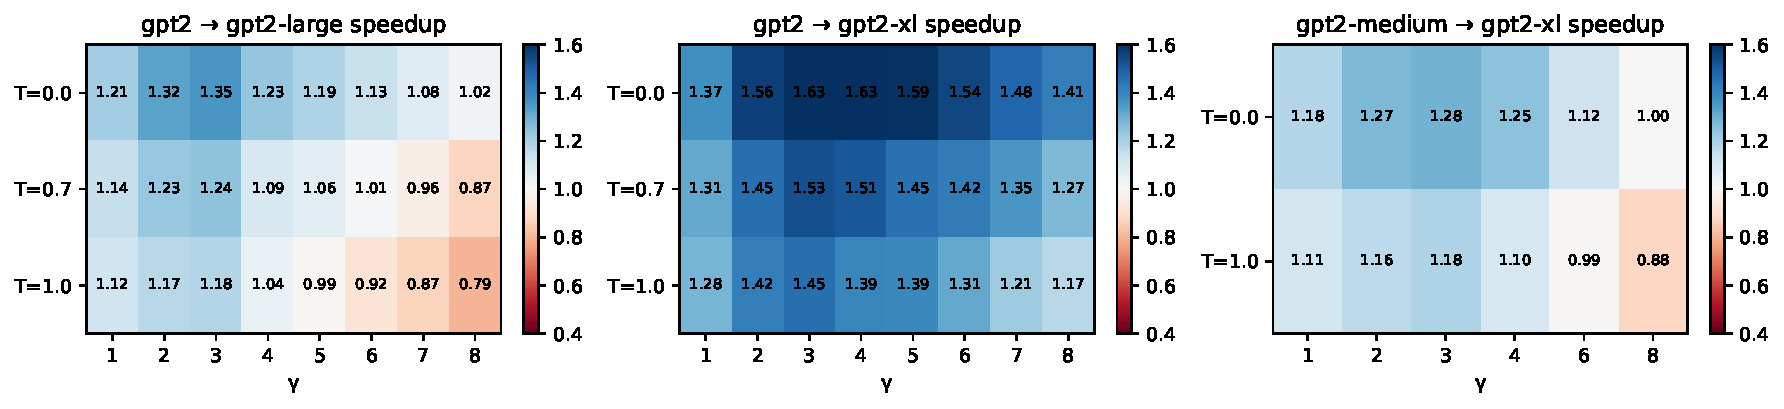
\includegraphics[width=\linewidth]{gpu_spec_heatmap.pdf}
\caption{加速热力图（行：温度，列：$\gamma$；蓝 $>1$，红 $<1$）。}\label{fig:heat}
\end{figure}

从 \cref{fig:speedup,fig:heat} 读出的规律：
\begin{itemize}
  \item \textbf{最优 $\gamma$ 很小}：两个 target 的最优点都在 $\gamma{=}3$--4，因为 $\alpha\approx0.64$--0.76 时 $\alpha^{\gamma}$ 衰减很快，多提议的 token 很少被接受，但每个都要付 $c$。
  \item \textbf{加速转为减速}：gpt2-large（$c{=}0.253$）在 $T{=}1$、$\gamma\ge5$ 时低于 1（0.986，$\gamma{=}8$ 时 0.794）；$T{=}0.7$ 在 $\gamma\ge7$ 时低于 1。gpt2-xl 的 $c$ 只有 0.138，
        $\gamma{=}8,T{=}1$ 仍有 1.165 倍。target 越大（$c$ 越小），可承受的 $\gamma$ 越大。
  \item \textbf{温度越高越差}：$T$ 升高使 $p$ 与 $q$ 的 TV 变大，$\alpha$ 下降约 0.07--0.08，所有 $\gamma$ 的加速都下降。
  \item \textbf{公式偏乐观 0--13\%}：60 个配置的实测 / 预测 = 0.87--1.00（gpt2-xl $\gamma{=}3,T{=}0$：1.631 / 1.688 = 0.966）。剩余差距是每轮一次 GPU→CPU 同步、
        Python 端拼 token 列表和 H2D 拷贝。\cref{eq:spec} 也没有计入 draft 补喂 2 个 token 那一步比 1 个 token 稍贵。
\end{itemize}

\textbf{更大的 draft 不一定更好}。补充实验用 gpt2-medium（355M）做 gpt2-xl 的 draft（60 个 prompt，$T\in\{0,1\}$）：贪心 $\hat\alpha$ 从 0.71 升到 0.77，
每次调用的 token 数也更多（$\gamma{=}3$：2.794 对 2.547），但 $c$ 从 0.138 涨到 0.308，最好的实测加速只有 1.283（$\gamma{=}3$，贪心），低于 gpt2 draft 的 1.631；
$T{=}1$ 时 $\gamma{=}6$ 已是 0.992，$\gamma{=}8$ 为 0.875。在 \cref{eq:spec} 中 $\alpha$ 从 0.71 提到 0.77 带来的收益，不够抵消 $\gamma c$ 翻倍的代价。
fp16 贪心一致性 54/60，分叉点 top-2 差同样 $\le 0.0078$。


\subsection{采样版推测解码不改变 target 分布}

在真实模型上做统计检验：draft gpt2、target gpt2-large、fp32、固定一个 64-token WikiText prompt、$\gamma{=}3$、每次生成 3 个 token，推测解码与 target 单独采样各重复 4000 次。
对第一个 token 可以算出精确的 target 分布 $p$ 与 draft 分布 $q$，把期望频数 $\ge5$ 的 token 单独成箱、其余合并后做卡方检验（\cref{tab:dist}）。

\begin{table}[H]
\centering\small
\caption{分布检验（\texttt{dist.jsonl}，每组 4000 次）}\label{tab:dist}
\begin{tabular}{lrrrrrr}
\toprule
温度 & $\mathrm{TV}(p,q)$ & 推测 vs $p$ & 推测 vs $q$ & 基线 vs $p$ & token 2 双样本 & token 3 双样本 \\
\midrule
$T=1.0$ & 0.269 & $p=0.657$ & $p=8.9\times10^{-168}$ & $p=0.096$ & $p=0.307$ & $p=0.499$ \\
$T=0.7$ & 0.101 & $p=0.182$ & $p=3.4\times10^{-124}$ & $p=0.752$ & $p=0.381$ & $p=0.034$ \\
\bottomrule
\end{tabular}
\end{table}

推测解码的第一个 token 与精确 $p$ 无显著差异（$p$ 值 0.657 / 0.182），却以 $10^{-124}$ 以下的 $p$ 值拒绝「来自 draft 分布 $q$」——检验有足够功效区分 $p$ 和 $q$。
第 2、3 个 token 没有闭式分布，用推测解码与 target 单独采样的双样本卡方检验比较；6 个双样本检验中最小 $p$ 值 0.034（$T{=}0.7$ 的第 3 个 token），
在 6 次检验的 Bonferroni 阈值 $0.05/6=0.0083$ 下不显著，与「6 次里出现一次 $p<0.05$」的偶然性一致。\Cref{fig:dist} 直观对比了 top-15 token 的频率。
（全词表的经验 TV 不是好指标：50{,}257 个 token 的长尾使 4000 次采样的 TV 噪声底就有 0.16，基线对精确 $p$ 也是 0.165。）

\begin{figure}[H]
\centering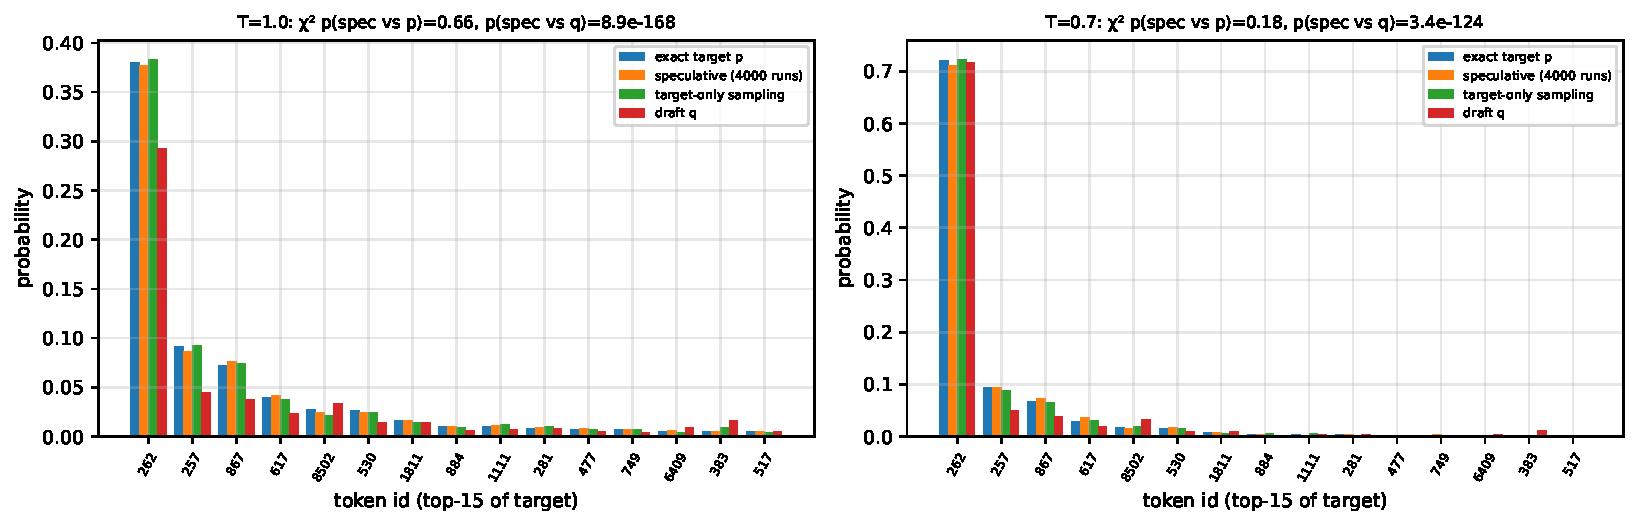
\includegraphics[width=\linewidth]{gpu_spec_distribution.pdf}
\caption{第一个生成 token 的分布（top-15）：精确 target $p$、推测解码频率、target 单独采样频率、draft $q$。}\label{fig:dist}
\end{figure}

\subsection{推测解码在大 batch 下为什么失效}

推测解码的前提是「验证 $\gamma{+}1$ 个 token 几乎和 1 个 token 一样贵」。\Cref{fig:cost} 在 batch $B$ 下测量 target 处理 $\gamma{+}1$ 个 token 的时间与单 token 的比值 $v(B)$，以及 $c(B)$（上下文 128）。
gpt2-xl 在 $B\le8$ 时验证 5 个 token 只贵 1.7--25\%，到 $B{=}128$ 时验证 9 个 token 是单 token 的 2.40 倍（27.53 对 11.47 ms）；draft 的 $c$ 在 $B\ge32$ 时也从 0.14 涨到 0.20--0.25，
因为 draft 自己开始出现 KV 读取与 GEMM 规模效应。

\begin{figure}[H]
\centering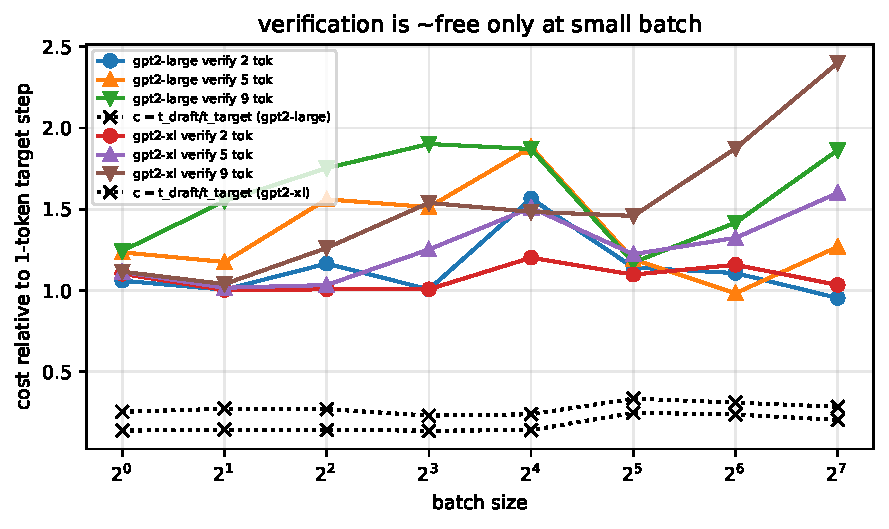
\includegraphics[width=0.7\linewidth]{gpu_spec_cost.pdf}
\caption{相对单 token target step 的代价：验证 2/5/9 个 token 的 $v(B)$，以及 draft 的 $c(B)$（黑点线）。}\label{fig:cost}
\end{figure}

把实测 $c(B)$、$v(B)$ 与主实验的 $\hat\alpha$ 代入 \cref{eq:spec}（\cref{fig:specbatch}，\texttt{spec\_batch\_model.csv}）：gpt2-xl、$T{=}1$、$\gamma{=}4$ 的预测加速从 $B{=}2$ 的 1.528 降到 $B{=}128$ 的 1.005；
$\gamma{=}8$ 在 $B\ge32$ 时低于 1（$B{=}128$ 为 0.674）。gpt2-large 在 $B{=}16$ 时出现一个低谷（$\gamma{=}4,T{=}1$ 为 0.926），对应 $v(16)=1.88$：
这一点上 $B(\gamma{+}1)=80$ 行的 GEMM 正好跨过了 cuBLAS 的 tile 边界。
\emph{注意这是用实测分量拼出的预测}，不是端到端测量：我们的 \texttt{SpecEngine} 只实现 batch 1（不同序列接受长度不同，需要 ragged KV 管理）。

\begin{figure}[H]
\centering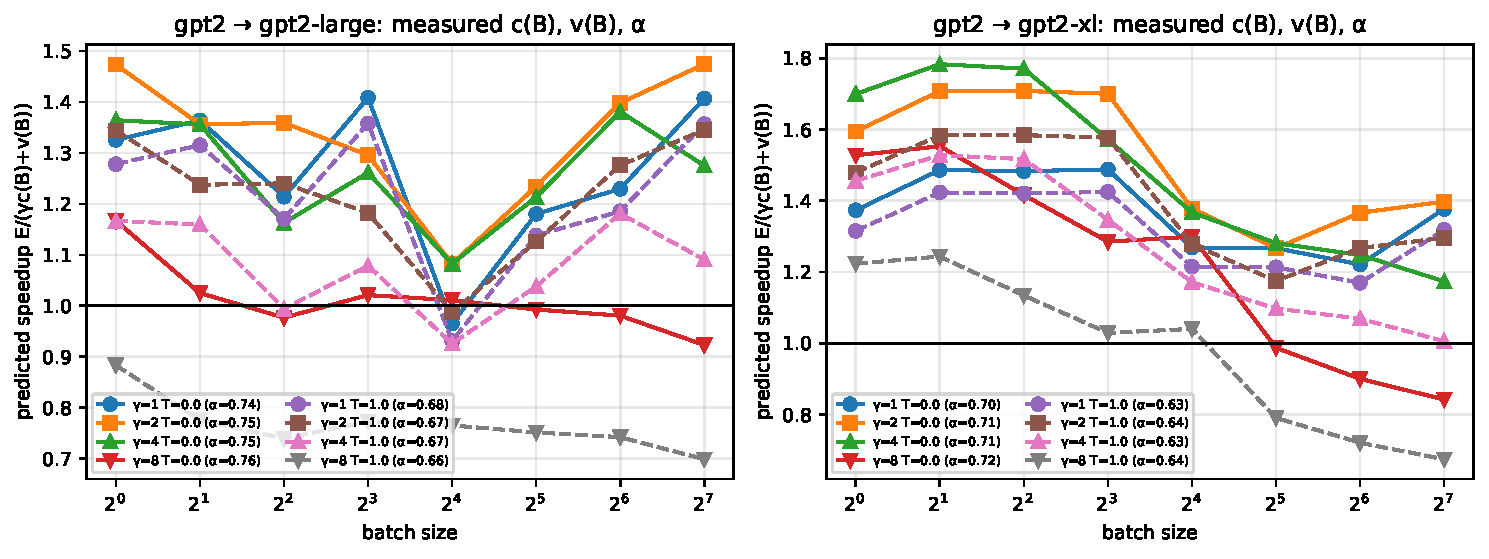
\includegraphics[width=\linewidth]{gpu_spec_batch.pdf}
\caption{用实测 $c(B)$、$v(B)$、$\hat\alpha$ 预测的推测解码加速 vs batch；黑线为 1。}\label{fig:specbatch}
\end{figure}

\begin{findingbox}[：推测解码什么时候不划算]
三个独立的失效方向都在数据里出现了：(1) $\gamma$ 太大（gpt2-large $T{=}1$，$\gamma{\ge}5$ 实测 $<1$）；(2) $\alpha$ 太低（温度从 0 到 1，$\alpha$ 降约 0.07，所有配置加速都下降）；
(3) batch 太大（gpt2-xl $\gamma{=}8$ 在 $B\ge32$ 时预测 $<1$），因为 decode 从 memory-bound 走向「验证不再免费」。
\end{findingbox}

\section{与理论模型的对照}

\subsection{decode 的 roofline}
一次 decode 读全部权重 $2N$ 字节（fp16）与全部 KV $2\cdot2LdTB$ 字节，做 $2NB + 4LdTB$ 次 FLOP。强度
\[
I(B) = \frac{2NB + 4LdTB}{2N + 4LdTB} \xrightarrow{T\to0} B, \qquad I(B)\xrightarrow{B\to\infty} 1 .
\]
所以不计 KV 时拐点在 $B^\star = P_{\text{peak}}/BW \approx 147$（实测峰值之比）；计入 KV 后，$B\to\infty$ 时强度趋于 1 FLOP/B，永远到不了 ridge。
GPT-2 没有 GQA，每 token KV 是 $4Ld$ 字节：gpt2-xl 为 300 KiB，相当于每 10{,}000 个 token 的上下文就是一份 3 GB 权重，这解释了上下文 256 下 batch 增大时 KV 很快主导。

\subsection{推测解码}
设每个 draft token 以独立概率 $\alpha$ 被接受，第一次拒绝前接受的个数 $K$ 服从截断几何分布 $P(K{=}k)=(1-\alpha)\alpha^k\ (k<\gamma)$，$P(K{=}\gamma)=\alpha^\gamma$，每轮产出 $K{+}1$ 个 token：
\[
\mathbb{E}[K+1] = \sum_{k=0}^{\gamma}\alpha^k = \frac{1-\alpha^{\gamma+1}}{1-\alpha}.
\]
$\alpha$ 的极大似然估计：每轮贡献「$K$ 次成功 + （若 $K<\gamma$）1 次失败」，似然 $\prod \alpha^{K}(1-\alpha)^{\mathbb{1}[K<\gamma]}$，
解得 $\hat\alpha = \sum K / (\sum K + \#\text{rejections})$，正是我们用的定义。对每一轮的耗时是 $\gamma c + v$（单位：target 单步），即 \cref{eq:spec}。
最优 $\gamma$ 满足 $\partial S/\partial\gamma=0$；以 gpt2-xl 贪心（$\alpha{=}0.71$，$c{=}0.138$，$v{\approx}1.11$）代入，$S(\gamma)$ 在 $\gamma{=}3,4$ 取得最大值 1.69--1.70，实测最优也在 $\gamma{=}3$--4（1.631 / 1.629）。

\subsection{分布无偏的证明}
对任意 token $x$：
\[
\begin{aligned}
P(\text{输出}=x) &= q(x)\min\!\Big(1,\frac{p(x)}{q(x)}\Big) + \Big(1-\sum_y \min(p(y),q(y))\Big)\frac{\max(p(x)-q(x),0)}{\sum_y\max(p(y)-q(y),0)} \\
&= \min(p(x),q(x)) + (p(x)-q(x))^+ = p(x),
\end{aligned}
\]
因为 $\sum_y(p-q)^+ = 1-\sum_y\min(p,q)$。贪心版是 $T\to0$ 的极限：$p$、$q$ 都退化成 one-hot，接受当且仅当 draft 的 argmax 等于 target 的 argmax。

\subsection{模型与实测的差距汇总}
\begin{table}[H]
\centering\small
\caption{模型 vs 实测}\label{tab:mvm}
\begin{tabularx}{\linewidth}{l r r X}
\toprule
量 & 模型 & 实测 & 差距来源 \\
\midrule
gpt2-xl decode，B=1，ctx 128 & 2.07 ms & 3.92 ms & 每层约 39 µs 的 kernel 固定开销 \\
gpt2-xl decode，B=256，ctx 256 & 15.27 ms & 20.00 ms & attention kernel 读 KV 达不到峰值带宽（比值 1.31）\\
KV 字节（58/63 组合） & 公式 & 逐字节相等 & 其余 5 个为 allocator 取整 \\
tokens/调用（采样） & $(1-\alpha^{\gamma+1})/(1-\alpha)$ & 相差 $<1\%$ & — \\
tokens/调用（贪心，$\gamma{=}8$） & 3.392 & 3.268 & $\alpha$ 跨上下文异质 \\
加速（gpt2-xl $\gamma{=}3$，贪心） & 1.688 & 1.631 & 每轮同步 + Python 开销 \\
\bottomrule
\end{tabularx}
\end{table}

\section{面试专题}

\subsection{20 秒电梯陈述}
我在 RTX 5090 上用真实 GPT-2 权重从零实现了 KV cache、CUDA Graph decode 和推测解码，fp32 下与 HF 的 logits 差 $\le 4.6\times10^{-5}$（大模型），贪心输出 bit-exact。
KV cache 在长上下文把 gpt2-xl 每 token 从 20.6 ms 降到 4.2 ms；但 batch 1 decode 只用到一半带宽，另一半是 per-kernel 开销。推测解码 gpt2→gpt2-xl 贪心实测 1.63 倍，
与 $(1-\alpha^{\gamma+1})/(1-\alpha)$ 加上实测 $c{=}0.138$、$v{=}1.11$ 的预测相差 4\%；并用数据展示了 $\gamma$ 过大、温度升高、batch 变大三种失效方式。

\subsection{STAR 故事}
\textbf{S}：推测解码的加速取决于 draft 相对代价 $c$，按参数量 gpt2/gpt2-xl 只有 0.08，理论加速应该很高。
\textbf{T}：解释为什么实测 $c$ 是 0.138，以及 decode 为什么只跑到 roofline 的一半。
\textbf{A}：在 4 个模型上测 batch 1 graph decode，把「实测 $-$ roofline」对层数作图，得到每层约 30--41 µs 的近似常数；再发现 SDPA+mask 在长上下文变慢，
把 decode attention 换成 bmm（沿 $T$ 切分），gpt2-xl 上下文 1024 从 6.36 ms 降到 4.22 ms。
\textbf{R}：用实测 $c$、$v$ 代入公式，60 个配置的实测 / 预测加速比在 0.87--1.00 之间，并准确预测了 gpt2-large 在 $\gamma\ge5$、$T{=}1$ 时转为减速。

\begin{iqbox}{为什么 decode 是 memory-bound，而 prefill 不是？}
decode 每步对每个权重只做 $B$ 次乘加，强度约 $B$ FLOP/B；5090 的 ridge 约 147 FLOP/B，batch 1 远低于它。prefill 一次处理 $P$ 个 token，强度约 $P$。实测 gpt2-xl prefill 512 个 token 12.80 ms，而 decode 1 个 token 就要约 4--5 ms。
\textbf{常见错答}：「因为 attention 是 $O(T^2)$」——decode 每步 attention 是 $O(T)$，batch 1 时主导的是读权重。
\end{iqbox}

\begin{iqbox}{KV cache 一定更快吗？}
不一定。实测 gpt2-xl 上下文 16 时 KV eager（6.21 ms）比无 cache（4.84 ms）慢，因为 batch 1 时 GPU 在等 CPU 发 kernel，KV 路径多出的小 kernel 反而增加了关键路径。
上下文 $\ge$128 才持平，1024 时快 3.3 倍（eager）/ 4.9 倍（graph+bmm）。
\textbf{常见错答}：「KV cache 永远是 $T$ 倍加速」——只在 compute 或访存真正成为瓶颈时成立。
\end{iqbox}

\begin{iqbox}{接受率 $\alpha$ 怎么估计？}
$\hat\alpha = \text{accepted}/(\text{accepted}+\text{rejections})$。一轮中第一次拒绝之后的 draft 从未被检验，不能计入分母。实测 gpt2→gpt2-xl $\gamma{=}8$：正确值 0.72，accepted/proposed 只有 0.28。
采样时 $\hat\alpha$ 应与 $\mathbb{E}[\sum\min(p,q)]$ 吻合（0.6285 对 0.6423）。
\textbf{常见错答}：用 accepted/proposed，然后发现公式「不准」。
\end{iqbox}

\begin{iqbox}{为什么采样版推测解码不改变分布？}
$P(x)=\min(p,q)+(1-\sum\min(p,q))\cdot\frac{(p-q)^+}{\sum(p-q)^+}=p(x)$。实测 4000 次对精确 $p$ 卡方 $p$ 值 0.657，对 $q$ 为 $8.9\times10^{-168}$。
\textbf{常见错答}：「拒绝后从 $p$ 重新采样」——那样 $x$ 会被重复计入，分布偏向 $q$ 与 $p$ 重叠的部分；必须从残差 $(p-q)^+$ 采样。
\end{iqbox}

\begin{iqbox}{draft 的 $c$ 为什么不是参数量之比？}
batch 1 decode 的时间 $\approx$ 权重字节 / 带宽 + 层数 $\times$ 每层固定开销。gpt2 只有 12 层但每层开销与大模型相同（约 30 µs），所以 gpt2 单步 0.56 ms，是 gpt2-xl（4.08 ms）的 0.138，而参数量之比是 0.08。
减小 $c$ 的办法：更浅的 draft、fuse kernel、或像 Medusa~\cite{medusa}/EAGLE 那样把 draft 头挂在 target 上。
\textbf{常见错答}：「$c$ = 参数比」。
\end{iqbox}

\begin{iqbox}{fp16 下推测解码的贪心输出为什么和 target 不完全一样？}
验证时 target 一次处理 $\gamma{+}1$ 个 token，GEMM 形状与单 token decode 不同，fp16 累加顺序不同。实测 gpt2-xl 100 个 prompt 中 9 个分叉，分叉点 top-2 logit 差最大 0.0078（fp16 ulp）。
fp32 下 120/120 完全一致。工程上用「平局容忍」或 batch-invariant kernel 解决。
\textbf{常见错答}：「推测解码在 fp16 下是有损的」——算法本身无损，差异来自数值，而且同样会出现在 KV vs 无 cache 之间。
\end{iqbox}

\begin{iqbox}{CUDA Graph 带来了什么，代价是什么？}
它把每步上千次 kernel launch 合成一次 replay：gpt2 单步从 1.56 ms 降到 0.49 ms。代价是形状固定：位置要做成 device 张量，attention 要在固定长度上加 mask；
如果固定为整块 $T_{\max}$，长上下文的 attention 成本会随 $T_{\max}$ 而不是实际长度增长（P=896 时 graph 810.5 ms 反而慢于 eager 794.6 ms）。实际系统按长度分桶 capture 多个 graph。
\textbf{常见错答}：「CUDA Graph 让 kernel 本身更快」——它只消掉 launch/CPU 开销。
\end{iqbox}

\begin{iqbox}{为什么大 batch 时推测解码收益下降？}
大 batch 下 decode 逐渐接近 compute-bound，验证 $\gamma{+}1$ 个 token 不再免费：gpt2-xl $B{=}128$ 时验证 9 个 token 是单 token 的 2.40 倍。代入公式 $\gamma{=}8,T{=}1$ 预测 0.674 倍。
所以 serving 系统通常在低负载时开推测解码，高负载时关掉或减小 $\gamma$。
\textbf{常见错答}：「batch 大了 $\alpha$ 会下降」——$\alpha$ 与 batch 无关，变的是 $v$ 与 $c$。
\end{iqbox}

\begin{iqbox}{KV cache 显存怎么算？}
$2\cdot L\cdot B\cdot H_{kv}\cdot d_h\cdot T\cdot\text{bytes}$。gpt2-xl fp16 每 token 300 KiB，$T{=}1024,B{=}32$ 为 10.07 GB，\texttt{memory\_allocated} 逐字节相等。
Llama-3-8B 用 GQA-8，每 token 只有 128 KiB（\texttt{inference\_math.csv}）。
\textbf{常见错答}：漏掉因子 2（K 和 V）或用 $H$ 而不是 $H_{kv}$。
\end{iqbox}

\section{局限}
\begin{caveatbox}
\begin{itemize}
  \item 推测解码只实现了 batch 1；大 batch 下的加速是用实测 $c(B)$、$v(B)$ 与 batch 1 的 $\hat\alpha$ 拼出来的预测，不是端到端测量。
  \item 所有计时都是单卡、fp16、PyTorch 算子级实现，没有 fused kernel / FlashDecoding / 量化；per-kernel 开销的结论针对这种实现，不代表 vLLM~\cite{vllm}/TensorRT-LLM 的绝对性能。
  \item $\alpha$ 来自 WikiText 的 100 个随机窗口，不同领域（代码、对话）的 $\alpha$ 可能差别很大；GPT-2 系列共享 tokenizer 与训练数据，$\alpha$ 偏高于一般异构模型对。
  \item 分布检验只覆盖一个 prompt 的前 3 个 token；它能发现明显的偏差，但不是对所有上下文的证明（证明见 \cref{sec:spec-res} 之后的推导与 CPU 版 60{,}000 次的显式 $p,q$ 检验）。
  \item GPU 与其他 6 个任务共享（用锁串行），计时取 20--30 次的中位数，但仍可能有频率/温度漂移；CPU 部分的计时受共享机器负载影响。
  \item fp16 的贪心一致性不是 bit-exact（gpt2-xl 91/100），我们只证明了分叉点是 fp16 平局。
\end{itemize}
\end{caveatbox}

\section{结论}
\begin{enumerate}
  \item \textbf{KV cache 的收益取决于瓶颈在哪里}。CPU 上它省掉的是 FLOP（T=1024 快 12.82 倍）；GPU batch 1 时短上下文的瓶颈是 kernel launch，eager KV 反而更慢，
        CUDA Graph 才把它变成真正的收益；长上下文时还要注意 decode attention 的并行度（SDPA+mask 对 bmm：6.36 对 4.22 ms）。
  \item \textbf{roofline 是下界不是预测}。gpt2-xl batch 1 实测是下界的 1.9 倍，差值是每层几十微秒的固定开销；大 batch 时比值降到 1.31，剩下的是 attention 读 KV 的效率。
  \item \textbf{推测解码的公式可以直接用来调参}，前提是 $\alpha$ 用正确的估计量、$c$ 和 $v$ 用实测值。用这三个数，公式对 60 个配置的预测与实测之比是 0.87--1.00，并正确指出了最优 $\gamma{=}3$--4 与减速区。
  \item \textbf{正确性要分精度讨论}：fp32 下所有「必须一致」都成立；fp16 下的分叉全部发生在 top-2 差 $\le$ 1 ulp 的平局处。采样版在真实模型上通过了对精确分布的卡方检验。
\end{enumerate}

\begin{thebibliography}{9}
\bibitem{leviathan} Y. Leviathan, M. Kalman, Y. Matias. Fast Inference from Transformers via Speculative Decoding. ICML 2023.
\bibitem{chen} C. Chen, S. Borgeaud, G. Irving, J.-B. Lespiau, L. Sifre, J. Jumper. Accelerating Large Language Model Decoding with Speculative Sampling. arXiv:2302.01318, 2023.
\bibitem{gpt2} A. Radford, J. Wu, R. Child, D. Luan, D. Amodei, I. Sutskever. Language Models are Unsupervised Multitask Learners. OpenAI, 2019.
\bibitem{pope} R. Pope et al. Efficiently Scaling Transformer Inference. MLSys 2023.
\bibitem{roofline} S. Williams, A. Waterman, D. Patterson. Roofline: An Insightful Visual Performance Model for Multicore Architectures. CACM 2009.
\bibitem{flashdec} T. Dao, D. Haziza, F. Massa, G. Sizov. Flash-Decoding for Long-Context Inference. 2023.
\bibitem{vllm} W. Kwon et al. Efficient Memory Management for Large Language Model Serving with PagedAttention. SOSP 2023.
\bibitem{medusa} T. Cai et al. Medusa: Simple LLM Inference Acceleration Framework with Multiple Decoding Heads. ICML 2024.
\bibitem{wikitext} S. Merity, C. Xiong, J. Bradbury, R. Socher. Pointer Sentinel Mixture Models. ICLR 2017.
\end{thebibliography}

\end{document}
